\documentclass{myreport}

\usepackage{longtable}

% % Change figure (table, section) numbering (e.g., from 'Figure 1' to 'Figure S1')
%  \renewcommand{\thefigure}{S\arabic{figure}}
%  \renewcommand{\thetable}{S\arabic{table}}
%  \renewcommand{\thesection}{S\arabic{section}}
%  \renewcommand{\theequation}{S\arabic{equation}}

\newcommand{\coo}{CO$_2$}

\begin{document}
\pagestyle{headings}

% Document must include
% ---------------------
% 

%% Title
\title{P-model evaluation}

\maketitle

\tableofcontents

%%%%%%%%%%%%%%%%%%%%%%%%%%%%%%%%%%%%%%%%%%%%%%%%%%%%%%%%
\section{Introduction}

\begin{itemize}
    \item Water-carbon trade-off, water use efficiency, $\chi = c_i:c_a$
    \item Acclimation, time scales
    \item Light use efficiency concept
    \item Optimality concept for predicting $\chi$ and LUE.
    \item Evaluation of predicted LUE and GPP (using prescribed greenness) with measured GPP at FLUXNET sites.
    \item Evaluation focuses on different components of variability (spatial, annual, seasonal, daily anomalies), functional relationships, and the response to drought.
    \item This paper describes the theory, the model implementation, and provides an comprehensive evaluation of predicted LUE and GPP with data from flux measurements.
    \item Model benchmarking is challenging in general due to errors introduced by uncertain model forcing data and by uncertainties in the observational data used for evaluation. We address these points here with an additional focus on uncertainties in the greenness data (model forcing), and uncertainties in the GPP data, derived from different flux decomposition methods, used for evaluation. 
    \item Sensitivities of processes to environmental conditions are key. It's generally challenging to derive them from continuous, not experimentally disturbed measurements. Here, we investigate functional relationships, determined from observations using Generalized Additive Models, and the response of LUE and GPP to drought, based on the soil moisture droughts detected by Stocker et al. (2018).
    \item General patterns in model-data mismatch. Additional simulations conducted to investigate whether these can be resolved.
    \item Value of this model is in providing a mechanistic and optimality-based LUE model that can be driven with observed greenness. Hence providing predicitions, grounded in basic ecological principles, and relying on a mimimum of prescribed model parameters.
\end{itemize}

\section{Methods}

\subsection{Theory}
\label{sec:theory}
The P-model centers around a prediction for the ratio of leaf-internal to ambient \coo ($c_i : c_a = \chi$) governed by the trade-off between the costs arising from the maintenance of carboxylation capacity ($V_{\mathrm{cmax}}$) and transpiration ($E$). 
It is founded on the standard model for C3 plant photosynthesis (Section \ref{sec:farquhar}), the coordination hypothesis (Section \ref{sec:coordination}) and the least-cost hypothesis (Section \ref{sec:least-cost}).

\textit{The following derivation and text is adopted and modified from Wang Han et al., 2017.}\\

\subsection{The standard model of C3 plant photosynthesis}
\label{sec:farquhar}
Following the Farquhar model for photosynthesis of C3 plants, instantaneous assimilation rates $A$ are limited either by the capacity of Rubisco for carboxylation of RuBP or the electron transport rate for the regeneration of RuBP. 
The Rubisco-limited photosynthetic rate $A_C$ is given by:
\begin{equation}
\label{eq:rubiscolimited}
    A_C = V_{\mathrm{cmax}} \; \frac{\chi\;c_a-\Gamma^{\ast}}{\chi\;c_a + K}
\end{equation}
where $V_{\mathrm{cmax}}$ is the Rubisco activity, $c_a$ is the ambient partial pressure of CO$_2$, $\chi$ is the ratio of leaf-internal to ambient CO$_2$ partial pressures, $\Gamma^{\ast}$ is the \coo\ compensation point in the absence of mitochondrial respiration, and $K$ is the effective Michaelis-Menten coefficient of Rubisco for carboxylation. 
Both $\Gamma^{\ast}$ and $K$ are influenced by the partial pressure of oxygen. 
$V_{\mathrm{cmax}}$, $\Gamma^{\ast}$ and $K$ are temperature-dependent, following Arrhenius kinetics.

The electron-transport limited photosynthetic rate $A_J$ is given by:
\begin{equation}
\label{eq:lightlimited}
    A_J = \phi_0 \; I\; \frac{\chi \; c_a - \Gamma^{\ast}}{\chi\;c_a + 2\Gamma^{\ast}}
\end{equation}
for low PPFD (I) where $\phi_0$ is the intrinsic quantum efficiency of photosynthesis. 
With increasing PPFD, $I$ must be substituted with a saturating function of the electron-transport capacity $J_{\mathrm{max}}$; various empirical functions have been used. 
The actual photosynthetic rate is then given by:
\begin{equation}
    A = \min(A_C, A_J)
\end{equation}

\subsubsection{The coordination hypothesis}
\label{sec:coordination}
Light use efficiency (LUE) models provide a powerful method and estimate assimilation rates as a linear function of absorbed light over a given time interval. 
But the connection between the Farquhar and LUE models is not obvious. 
Equation \ref{eq:lightlimited} predicts that electron-transport limited photosynthesis is proportional to absorbed PPFD but only applies at relatively low PPFD, and in any case, Equation \ref{eq:rubiscolimited} for Rubisco-limited photosynthesis is expected to apply at high PPFD. 
The conundrum is this: how can GPP (the time-integral of photosynthesis) be proportional to PPFD, which is the basis of the LUE model, if the response of photosynthesis to PPFD saturates, as it should according to the Farquhar model? This question has surfaced occasionally in the literature, but not been fully resolved. 
Medlyn10 reviewed some alternative explanations.
 
One of the explanations discussed by Medlyn10 invokes the co-ordination (or co-limitation) hypothesis, which states that $V_{\mathrm{cmax}}$ of leaves at any level in the canopy acclimates spatially and temporally to the prevailing daytime incident PPFD in such a way as to be neither in excess (entailing additional, futile maintenance respiration), nor less than required for full exploitation of the available light. 
In other words, under typical daytime condition when most photosynthesis takes place, the following is valid:
\begin{equation}
\label{eq:coordination}
    A_J \approx A_C
\end{equation}
This hypothesis also requires that $J_{\mathrm{max}}$ maintain a ratio to $V_{\mathrm{cmax}}$ such that strong limitation by $J_{\mathrm{max}}$ is avoided. 
Evidence for the co-ordination hypothesis was presented by Haxeltine and Prentice11, and Dewar12, who noted that it can explain many otherwise unexplained responses of C3 plants to environmental changes: including changes in leaf C:N ratios along environmental gradients, and the widely observed reduction of $V_{\mathrm{cmax}}$ under experimentally increased atmospheric CO2. More recently Maire et al.13 showed very good agreement between typical daytime values of $A_J$ and $A_C$ as calculated under the prevailing growth conditions for 31 species (293 data points) based on published studies. 
The co-ordination hypothesis allows a simple approximation by which equation S2 is applied to predict GPP over time scales for which acclimation of $V_{\mathrm{cmax}}$ is possible, with $I$ now representing daily, rather than instantaneous, PPFD.

\subsubsection{The least-cost hypothesis}
\label{sec:least-cost}
Missing from the Farquhar model is an equation to predict χ, which constrains both the Rubisco- and electron-transport limited rates of carbon fixation and therefore appears in both equations S1 and S2. 
$\chi$ at any moment must be consistent both with the rate of carbon fixation and with the rate of diffusion of \coo\ through the stomata. 
Although the mechanism of stomatal control is still an active research topic, there is abundant evidence that $\chi$ is closely regulated to remain within a narrow range. 
All current Earth System Models include a 'closure' that predicts either stomatal conductance or $\chi$. 
The most commonly used closures are the one-parameter Ball-Berry equation14 and the two-parameter Leuning equation15 (or equivalently, the ‘Jacobs closure’16). 
Both are empirical, and incomplete in the sense that they allow $\chi$ to react only to relative humidity (Ball-Berry) or VPD (Leuning/Jacobs). 
Although superficially similar, these equations make substantially different predictions. 
For example, Ball-Berry allows $\chi$ to approach unity as VPD tends to zero, whereas Leuning/Jacobs caps $\chi$ at a maximum value. 
Both equations are usually implemented with different parameter values for different PFTs, but with no strong basis for the distinctions.

The least-cost hypothesis by Prentice et al. (2014), first proposed by Wright et al. (2003), states that $\chi$ should minimize the combined cost (per unit of assimilation) of maintaining the capacities for carboxylation and transpiration. 
If $a$ and $b$ are dimensionless cost factors (maintenance respiration per unit assimilation) for the maximum rates of water transport ($E$) and carbon fixation ($V_{\mathrm{cmax}}$) respectively, the optimality criterion is:
\begin{equation}
\label{eq:leastcost}
    a \; \frac{\partial (E/A)}{\partial \chi} = -b \; \frac{\partial (V_{\mathrm{cmax}}/A)}{\partial \chi}
\end{equation}

\subsubsubsection{Predicting $\chi$}
The following section provides a derivation of optimal $\chi$ using Fick's Law, above stated hypotheses and the Farquhar model for C3 photosynthesis. 
Transpiration $E$ and assimilation $A$ are coupled through stomatal conductance ($g_s$).
According to the Fick's Law of diffusion:
\begin{align}
\label{eq:fick}
    E &= 1.6 \; g_s \; D \\
    A &= g_s \; c_a \; (1-\chi)
\end{align}
Therefore,
\begin{equation}
    E/A = \frac{1.6 \; D}{c_a\;(1-\chi)}
\end{equation}
The derivative term on the left-hand-side of Eq.\label{eq:leastcost} can thus be written as
\begin{equation}
\label{eq:partial1}
    \frac{\partial (E/A)}{\partial \chi} = \frac{1.6\;D}{c_a\;(1-\chi)^2}\;.
\end{equation}
Using Equation \ref{eq:rubiscolimited} and the simplification $\Gamma^{\ast}=0$, the derivative term on the right-hand-side of Eq.\label{eq:leastcost} can be written as
\begin{equation}
\label{eq:partial2}
    \frac{\partial (V_{\mathrm{cmax}}/A)}{\partial \chi} = - \frac{K}{c_a\;\chi^2}
\end{equation}
Using equations \ref{eq:partial1} and \ref{eq:partial2}, Eq. \ref{eq:leastcost} can be written as
\begin{equation}
    a\;\frac{1.6\;D}{c_a\;(1-\chi)^2} = b\;\frac{K}{c_a\;\chi^2}
\end{equation}
and solved for $\chi$:
\begin{align}
    \chi &= \frac{\xi}{\xi + \sqrt{D}} \\ 
    \xi &= \sqrt{\frac{b\;K}{1.6\;a}}
\end{align}
The exact solution, without the simplification $\Gamma^{\ast}=0$, is 
\begin{align}
\label{eq:chi_exact}
    \chi &= \frac{\Gamma^{\ast}}{c_a} + \left(1- \frac{\Gamma^{\ast}}{c_a}\right)\;\frac{\xi}{\xi + \sqrt{D}}\\
    \xi &= \sqrt{\frac{b(K+\Gamma^{\ast})}{1.6\;a}}
\end{align}
This can also be written as
\begin{equation}
\label{eq:ci}
    c_i = \frac{\Gamma^{\ast}\sqrt{D}+ \xi\;c_a}{\xi + \sqrt{D}} \\ 
\end{equation}
\clearpage

With this prediction for $c_i$, acclimated at a time scale on the order of weeks, the assimilation rate, Eq. \ref{eq:lightlimited} can be used in the sense of a light use efficiency model, whereby the total assimilation is proportional to the total absorbed PPFD over a given time interval:
\begin{equation}
\label{eq:lue}
        A_J = \phi_0 \; I_{\mathrm{abs}}\;\underbrace{\frac{c_i - \Gamma^{\ast}}{c_i + 2\Gamma^{\ast}}}_{m}
\end{equation}
Using Eq. \ref{eq:ci} and $\beta=b/a$, $m$ can be written as
\begin{equation}
    m = \frac{c_a - \Gamma^{\ast}}{c_a + 2 \Gamma^{\ast} + 3 \Gamma^{\ast} \sqrt{\frac{1.6 \eta^{\ast} D }{\beta\;(K+\Gamma^{\ast})}}}
\end{equation}
This provides an expression for predicting the assimilation rate from first principles as a function of temperature, moisture (vapour pressure deficit $D$), elevation and atmospheric CO$_2$ partial pressure.

\subsubsection{Introducing $J_{\mathrm{max}}$ limitation}
Equation \ref{eq:lue} is correct only if the response of GPP ($A$) to increasing PPFD remains linear up to the co-limitation point. 
By considering a non-rectangular hyperbola relationship between $A_J$ and $I_{\mathrm{abs}}$ (ref 26), we allow for the effect of finite $J_{\mathrm{max}}$:
\begin{equation}
\label{eq:ajlim}
    A_J = \phi_0 \; I_{\mathrm{abs}} \; m \; \underbrace{ \frac{1}{\sqrt{1+ \left( \frac{4\;\phi_0\;I_{\mathrm{abs}}}{J_{\mathrm{max}}} \right)^{2}}} }_{L}
\end{equation}
In the following, we aim for an expression of the limitation factor $L$ as a function of a $J_{\mathrm{max}}$ cost factor $c^{\ast}$. 
We define two dimensionless quantities, $a_0$ and $k$:
\begin{equation}
\label{eq:a0}
    a_0 = \frac{J_{\mathrm{max}}}{4\;\phi_0\;I_{\mathrm{abs}}}
\end{equation}
\begin{equation}
    k = \frac{J_{\mathrm{max}}}{4\;V_{\mathrm{cmax}}}\;.
\end{equation}
The model equations for $A_J$ and $A_C$ can then be re-written as:
\begin{equation}
\label{eq:ajlim2}
    A_J = \phi_0 \; I_{\mathrm{abs}} \; \; \frac{c_i - \Gamma^{\ast}}{c_i + 2\Gamma^{\ast}} \frac{1}{\sqrt{1+a_0^{-2}}}
\end{equation}
and
\begin{equation}
    A_C = \frac{J_{\mathrm{max}}}{4\;k} \cdot \frac{c_i - \Gamma^{\ast}}{c_i + K}
\end{equation}
Under the assumption of the coordination hypothesis, we set again $A_J = A_C$ and solve for $k$ to define the ratio of $J_{\mathrm{max}}$ to $V_{\mathrm{cmax}}$:
\begin{equation}
\label{eq:k}
    k = \frac{c_i + 2\Gamma^{\ast}}{c_i + K} \; \sqrt{a_0^2 + 1}
\end{equation}
Solving Eq. \ref{eq:k} for $a_0$ and substituting this into Eq. \ref{eq:ajlim} we can express the $J_{\mathrm{max}}$ limitation factor $L$ as:
\begin{equation}
\label{eq:ajlim3}
    L = \frac{1}{\sqrt{1 - \left( \frac{c_i+2\Gamma^{\ast}}{k(c_i+K)} \right)^{2}}}
\end{equation}

To obtain an estimate of the optimum value of $J_{\mathrm{max}}$ we assume that (a) there is a cost associated with $J_{\mathrm{max}}$ that is equal to the product of $J_{\mathrm{max}}$ and a constant $c$, and (b) that the value of $J_{\mathrm{max}}$ maximizes the benefit ($A_J$) minus the cost. 
This maximum is obtained when
\begin{equation}
\label{eq:jmaxpartial}
    \frac{\partial A_J}{\partial a_0} = c \; \frac{\partial J_{\mathrm{max}}}{\partial a_0}\;.
\end{equation}
Using Eq. \ref{eq:ajlim2}, the left-hand-side of Eq. \ref{eq:jmaxpartial} is 
\begin{equation}
    \frac{\partial A_J}{\partial a_0} = \phi_0 \; I_{\mathrm{abs}} \; \; \frac{c_i - \Gamma^{\ast}}{c_i + 2\Gamma^{\ast}} \left( a_0^{-2} + 1 \right) ^{-2/3} a_0^{-3}
\end{equation}
Using Eq. \ref{eq:a0}, the right-hand-side of Eq. \ref{eq:jmaxpartial} is 
\begin{equation}
    \frac{\partial J_{\mathrm{max}}}{\partial a_0} = 4 \; \phi_0 \; I_{\mathrm{abs}}\;.
\end{equation}
Now, we can solve Eq. \ref{eq:jmaxpartial} for $a_0^2$:
\begin{equation}
\label{eq:a0}
a_0^2 = \frac{(c_i - \Gamma^{\ast})^{2/3}}{c^{2/3} \; (c_i+2\Gamma^{\ast})^{2/3}}-1
\end{equation}
and use this in Eq. \ref{eq:k} to solve for $k^2$:
\begin{equation}
\label{eq:k2}
k^2 = (c_i+ \Gamma^{\ast})^{4/3} \; (c_i - \Gamma^{\ast})^{2/3} \; (c_i + K)^{-2} \; c^{-2/3}
\end{equation}
and for $c$:
\begin{equation}
\label{eq:c}
    c = \frac{(c_i+2\Gamma^{\ast})^2\;(c_i-\Gamma^{\ast})}{k^3\;(c_i+K)^3}
\end{equation}
Eq. \ref{eq:k2} can be plugged into Eq. \ref{eq:ajlim3} to express $L$ as
\begin{equation}
    L = \sqrt{1-c^{2/3} \; \left( \frac{c_i+2\Gamma^{\ast}}{c_i-\Gamma^{\ast}}\right)^{2/3}  }
\end{equation}
Using the prediction of $c_i$ from Eq. \ref{eq:ci}, this can be written as
\begin{equation}
    L =  \sqrt{1 - \left( \frac{c}{m} \right)^{2/3} }
\end{equation}
The revised LUE model thus becomes
\begin{equation}
\label{eq:ajlim4}
    A_J = \phi_0 \; I_{\mathrm{abs}} \; m'
\end{equation}
with
\begin{equation}
    m' = m \; \sqrt{1 - \left( \frac{c}{m} \right)^{2/3} }
\end{equation}
Taking typical values of $k$ = 0.4726 and $\chi$ = 0.820, we estimate (using Eq. \ref{eq:c}) c = 0.41.

% \subsubsection{Corollary of the $\chi$ prediction}
% \subsubsubsection{Stomatal conductance}
% Stomatal conductance $g_s$ follows from the prediction of $\chi$ given by Eq. \ref{eq:chi_exact} and $g_s = A / ( c_a\;(1-\chi) )$ (from Eq. \ref{eq:fick}). Stomatal contuctance can thus be written as
% \begin{equation}
%     g_s = \left( 1 + \frac{\xi}{\sqrt{D}} \right) \frac{A}{c_a}
% \end{equation}
% This is equivalent to the form derived by Medlyn et al., 2011, apart from the $g_0$ parameter that is missing here.

% $g_s$ also follows from the predictions of $A$ and $ci$, using Eq. \ref{eq:fick}. The stomatal conductance to water vapour (not CO$_2$) is:
% \begin{equation}
% g_s^W = \frac{1.6 \; p\; A}{c_a - c_i}
% \end{equation}
% With $g_s^W$ commonly expressed in units of mol H$_2$O m$^{-2}$ s$^{-1}$, $g_s$ in P-model being the stomatal conductance to CO$_2$, and $c_i$ (and $c_a$) defined as CO$_2$ partial pressure in units of Pa, multiplication with atmospheric pressure $p$ (Pa) and the factor 1.6 to convert stomatal conductance to CO$_2$ into stomatal conductance to H$_2$O are required.

% Note that in the P-model output, $c_i$ is given in ppm.

% \subsubsubsection{Intrinsic water use efficiency}
% The intrinsic water use efficiency (iWUE) is defined as the ratio of assimilation over stomatal conductance (to water). With Eq. \ref{eq:fick} this is
% \begin{equation}
%     \mathrm{iWUE} = A / g_s^W = \frac{c_a - c_i}{1.6\;p}
% \end{equation}
% With $A$ expressed in units of mol CO$_2$ m$^{-2}$ s$^{-1}$, and $g_s^W$ in units of mol H$_2$O m$^{-2}$ s$^{-1}$, iWUE is unitless. The factor 1.6 accounts for the difference in diffusivity between CO$_2$ and H$_2$O. In all above calculations, $c_a$ and $c_i$ are expressed as partial pressure of CO$_2$ in units of Pa. Division by the atmospheric pressure $p$ converts $(c_a - c_i)$ to unitless.


% \subsubsubsection{$V_{\mathrm{cmax}}$}

% Rearranging Eq. \ref{eq:rubiscolimited} and $\gamma=\Gamma^{\ast}/c_a$ and $\kappa=K/c_a$ gives
% \begin{equation*}
%     V_{\mathrm{cmax}} = A_C\;\frac{\chi+\kappa}{\chi-\gamma}
% \end{equation*}
% With the coordination $A_J=A_C$ (Eq. \ref{eq:coordination}) and Eq. \ref{eq:lue}, $V_{\mathrm{cmax}}$ can be written as
% \begin{equation}
%     \label{eq:vcmax}
%     V_{\mathrm{cmax}} = \phi_0\;I_{\mathrm{abs}}\;\frac{\chi+\kappa}{\chi+2\gamma}
% \end{equation}
% %Normalising to standard temperature (25$^{\circ}$C) gives $V_{\mathrm{cmax25}}$ as
% %\begin{equation}
% %    V_{\mathrm{cmax25}} = V_{\mathrm{cmax}} \; \exp\Bigg(\frac{\Delta H_{\mathrm{Vcmax}}}{R}\Big( \frac{1}{T_{K25}} - \frac{1}{T_K} \Big)\Bigg)
% %\end{equation}
% %with $\Delta H_{\mathrm{Vcmax}}=65330$ J mol$^{-1}$, $R = 8.3145$ J mol$^{-1}$ K$^{-1}$, $T_K$ is the ambient temperature in Kelvin, and $T_{K25}$ is 25$^{\circ}$C in Kelvin (298.15 K).
% %Wang Han (in prep.) implemented this as
% Normalising to standard temperature (25$^{\circ}$C) gives $V_{\mathrm{cmax25}}$ as
% \begin{equation}
% \label{eq:vcmaxsens}
%     V_{\mathrm{cmax25}} = V_{\mathrm{cmax}}\; f_V^{-1}  = V_{\mathrm{cmax}} \; \Bigg( \exp\Big( \frac{H_a(T_K-T_{K25})}{T_KT_{K25}R}\;\frac{1+\exp( \frac{T_{K25}\Delta S-H_d}{RT_{K25}} )}{1+\exp( \frac{T_K\Delta S - H_d}{RT_K} )} \Big) \Bigg)^{-1}
% \end{equation}
% with $H_a$ being the activation energy (71513 J mol$^{-1}$), $R$ is the universal gas constant (8.3145 J mol$^{-1}$ K$^{-1}$), $T_K$ is the ambient temperature in Kelvin, and $T_{K25}$ is 25$^{\circ}$C in Kelvin (298.15 K). $H_d$ is the deactivation energy (200000 J mol$^{-1}$), and $\Delta S$ is an entropy term (J mol$^{-1}$ K$^{-1}$) calculated using a linear relationship with $T$ from Kattge and Knorr (2007), with a slope of 1.07 J mol$^{-1}$ K$^{-2}$ and intercept of 668.39 J mol$^{-1}$ K$^{-1}$. 
% %Wang Han (in prep.) implemented this as
% %\begin{equation}
% %    V_{\mathrm{cmax25}} = V_{\mathrm{cmax}} \; \exp\Bigg( \frac{H_a(T-T_{\text{ref}})}{T_{\text{ref}}TR}\;\frac{1+\exp( \frac{T_{\text{ref}}\Delta S - H_d}{RT_{\text{ref}}}  )}{1+\exp( \frac{T\Delta S-H_d}{RT} )} \Bigg)
% %\end{equation}

% \subsubsubsection{Dark respiration $R_{\mathrm{d}}$}

% Dark respiration at standard temperature $R_{\mathrm{d25}}$ is calculated as being proportional to $V_{\mathrm{cmax25}}$:
% \begin{equation}
% \label{eq:rd25}
%     R_{\mathrm{d25}} = b_0 \; V_{\mathrm{cmax25}}
% \end{equation}
% where $b_0 = 0.014$. 
% Dark respiration follows a different temperature sensitivity. Following Heskel et al. (2016):
% \begin{equation}
% \label{eq:rdsens}
%     R_{\mathrm{d}} =  R_{\mathrm{d25}}\; f_R  = R_{\mathrm{d25}} \exp \Big(  0.1012(T_{K25}-T_K) - 0.0005(T_{K25}^2-T_K^2) \Big) 
% \end{equation}
% By combining Equations \ref{eq:vcmaxsens}, \ref{eq:rd25}, and \ref{eq:rdsens}, $R_d$ at growth temperature $T$ can directly be calculated from $V_{\mathrm{cmax}}$
% \begin{equation}
%     R_d = b_0 \frac{f_R}{f_V}\;V_{\mathrm{cmax}}
% \end{equation}

%Dark respiration at ambient temperature follows a sensitivity with a different activation energy than $\Delta H_{\mathrm{Vcmax}}$:
%\begin{equation}
%    R_{\mathrm{d}} = R_{\mathrm{d25}} \Bigg( \exp\Bigg(\frac{\Delta H_{\mathrm{Rd}}}{R}\Big( \frac{1}{T_{K25}} - \frac{1}{T_K} \Big)\Bigg) \Bigg)^{-1}
%\end{equation}

\subsubsection{The light use efficiency model}
\label{sec:luemodel}
For the further model description, we refer to ecosystem-scale quantities and 

\begin{equation}
\text{GPP} = \text{fAPAR} \cdot \text{PPFD} \cdot \text{LUE}
\label{eq:luemodel}
\end{equation}
with 
\begin{align}
    \text{GPP} &= A_J \\
    \text{fAPAR} \cdot \text{PPFD} &= I_{\text{abs}} \\
    \text{LUE} &= \beta(\theta) \; \phi_0(T) \; m'
\end{align}

\paragraph{Temperature dependence}
The temperature dependence of quantum yield efficiency ($\phi_0(T)$) is modelled following the temperature dependence of the maximum quantum yield of photosystem II in light-adapted tobacco leaves, determined by Bernacchi et al., 2003 (xxx add bibref) as 
\begin{equation}
\phi_0(T) = a_T \; b_T \; ( 0.352 + 0.022\;T - 0.00034\;T^2 )
\end{equation}
where $a_T$ is the leaf absorptance, and $b_T$ is the fraction of absorbed light that reaches photosystem II. $(a_T \cdot b_T)$ is treated as a single calibratable parameter (see Section \ref{sec:calib}), and further referred to as $\widehat{c_T}\equiv a_t\;b_b$. Note that the temperature dependence of quantum yield efficiency was not accounted for in earlier publications with the P-model (xxx refs) and $\phi_0$ was treated as a constant. Here, we conducted simulations both with constant and temperature-dependent $\phi_0$. For the former, $\phi_0$ was treated as a single calibratable parameter (below referred to as $\widehat{\phi_0}$), and implicitly includes the factors for leaf absorbtance, light attenuation before reaching chloroplasts. Both $\widehat{c_T}$ and $\widehat{\phi_0}$ implicitly account for incomplete utilization of the spectrum of incident PPFD.

\paragraph{Soil moisture stress}
$\beta(\theta)$ is a soil moisture stress function. We use results by Stocker et al. (2018) (xxx add bibref) to fit a soil moisture stress functions ($\beta(\theta)\simeq\text{fLUE}$) based on two general patterns. First, the functional form of $\beta(\theta)$ can be approximated by a quadratic function that approaches 1 for soil moisture above a certain threshold $\theta^{\ast}$ and held constant at 1 for soil moisture values above that. Here $\theta$ is the plant-available soil water, expressed as a fraction of field capacity. The general form is:
\begin{equation}
    \beta =
\begin{cases}
    q(\theta - \theta^{\ast})^2 + 1,& \theta \leq \theta^{\ast}\\
    1,              & \theta > \theta^{\ast}
\end{cases}
\end{equation}
Second, the sensitivity of $\beta(\theta)$ to extreme soil dryness ($\theta \rightarrow 0$) is related to the mean aridity. The dryness-related decline in $\beta(\theta)$ is particularly strong in driest climates, whereas a smaller reduction in $\beta(\theta)$ when soil water gets depleted is recorded at intermediate aridity. In the equation above, the sensitivity parameter $q$ is defined by the maximum $\beta$ reduction at low soil moisture $\beta_0\equiv\beta(\theta=\theta_0)$, leading to $q=(\beta_0-1)/(\theta^{\ast}-\theta_0)^2$. Note that $q$ has a negative value. $\beta_0$ is modelled as a linear function of the mean aridity, quantified by the mean annual ratio of AET/PET:
\begin{equation}
\beta_0 = \widehat{a_{\theta}} + \widehat{b_{\theta}} (\text{AET}/\text{PET})
\end{equation}
$\widehat{a_{\theta}}$ and $\widehat{b_{\theta}}$ are treated as calibratable parameters. 

Soil moisture ($\theta$) was simulated using the SPLASH model, which treats soil water storage as a single bucket and calculates potential evapotranspiration based on Priestly-Taylor (xxx ref). Here, we account for a variable water holding capacity calculated based soil porosity and depth data from SoilGrids (xxx ref, see Appendix XXX). The soil water balance model is described in detail in xxx ref Davis. 

\begin{table}
\centering
\begin{tabular}{llll}
	\toprule
    Symbol     & Value     &  Description   &  Reference   \\
	\midrule
    \beta      & 146       &  Ratio of unit costs, Eq. xxx   &  xxxx   \\
	\bottomrule
\end{tabular}
\caption{Model parameters used for all setups.}
\label{tab:params}
\end{table}

\subsection{Simulation protocol}
\label{sec:protocol}
To investigate model performance in dependence of alternative choices for model forcing data (defining fAPAR), alternative model setups (variable/fixed soil moisture and temperature effects), and alternative observational target data for calibration (GPP based on different flux decompositions), we conducted multiple simulation sets. Parameters ($\widehat{c_T}$, $\widehat{a_{\theta}}$, and $\widehat{b_{\theta}}$) are calibrated and evaluated against respective observational data for each simulation set separately.

The simulation set ORG corresponds to the model as used in xxx ref Wang Han et al., 2017. That is, the quantum efficiency of photosynthesis ($\widehat{\phi_0}$) is fixed, and without accounting for soil moisture stress ($\theta=1$). The model is forced with fAPAR data taken as MODIS FPAR, splined to daily values (see also Section \ref{sec:greennessdata}, and calibrated against GPP data from FLUXNET 2015 based on the nighttime decomposition method ('NT'). All simulation setups are described in Tab. \ref{tab:setups}. The simulation set BRC is identical to ORG, except that  $\widehat{\phi_0}$ is allowed to vary with temperature. In the simulation set FULL, soil moisture stress is additionally accounted for.

Additional simulations account for both temperature and soil moisture effects. The simulation set FULL\textunderscore FPARitp also uses MODIS FPAR (MCD15A3H) data for fAPAR, but with daily values as linear interpolations of original data, which is given for 4-day intervals. This is used to investigate whether the smoothed values of the splined data (standard) are responsible for the general underestimation of maximum GPP values during the height of the growing season. The simulation set FULL\textunderscore EVI uses MODIS EVI (MOD13Q1), splined to daily from 8-daily data, to assess to which degree model performance depends on fAPAR forcing data. See Section \ref{sec:greennessdata} for more information.

Additional simulation sets FULL\textunderscore DT, FULL\textunderscore NTsub, and FULL\textunderscore Ty are used to investigate the dependence of (apparent) model performance on the observational data source to which it is calibrated. Here, the model is calibrated to GPP data derived using different CO$_2$ flux decomposition methods. We use GPP data based on the nighttime decomposition method (xxx ref reichstein) for FULL\textunderscore NTsub, the daytime decomposition method (xxx ref) for FULL\textunderscore DT, and an alternative decomposition method used for model-data comparison in Wang Han et al., 2017 (xxx ref) for FULL\textunderscore Ty. The latter method determines a constant background respiration rate as the (fitted) asymptote of CO$_2$ exchange fluxes with PPFD tending towards zero. This data is publicly available at XXX. Calibration and evaluation of FULL\textunderscore DT, FULL\textunderscore NTsub, and FULL\textunderscore Ty are done only for sites and dates where observational data is given from all three datasets (DT, NT, and Ty), hence the distiction between FULL\textunderscore NTsub and FULL. The model calibration is implemented within the rsofun R package (function \texttt{calib\textunderscore sofun()}, see accompanying paper Stocker et al., XXX).

\begin{table}
\resizebox{\textwidth}{!}{%
\begin{tabular}{lllllllll}
	\toprule
    Setup name                 &  fAPAR data              &  GPP      &  Calibration set  &  SM limit.  &  \widehat{\phi_0} &  \widehat{c_T}    &  $\widehat{a_{\theta}}$  &  $\widehat{b_{\theta}}$   \\
	\midrule
    ORG                        &  FPAR MCD15A3H, spl.     &  NT       &  valid NT data    &  no         &  0.0500 &  --     &  -- & --   \\
    BRC                        &  FPAR MCD15A3H, spl.     &  NT       &  valid NT data    &  no         &  --     &  0.0832 &  -- & --   \\
    FULL                       &  FPAR MCD15A3H, spl.     &  NT       &  valid NT data    &  yes        &  --     &  0.0885 &  0  & 0.687 \\
	\midrule
    FULL\textunderscore FPARitp &  FPAR MCD15A3H, itpl.   &  NT       &  valid NT data    &  yes        &  --     &  0.0860 &  0  & 0.700 \\
    FULL\textunderscore EVI     &  EVI MOD13Q1, spl.      &  NT       &  valid NT data    &  yes        &  --     &  0.1317 &  0  & 0.770 \\
	\midrule
    FULL\textunderscore DT      &  FPAR MCD15A3H, spl.    &  DT       &  valid NT, DT, Ty &  yes        &  --     &  0.0909 & 0   & 0.690 \\
    FULL\textunderscore Ty      &  FPAR MCD15A3H, spl.    &  Ty       &  valid NT, DT, Ty &  yes        &  --     &  0.0886 & 0   & 0.722 \\
    FULL\textunderscore NTsub   &  FPAR MCD15A3H, spl.    &  NT       &  valid NT, DT, Ty &  yes        &  --     &  0.0918 & 0   & 0.688 \\
	\bottomrule
\end{tabular}}
\caption{Model setups. The standard greenness data, used to define the model forcing for fAPAR is MODIS FPAR MCD15A3H (xxx ref), where the original data, given at 4-day intervals, is splined to daily values (see Section \ref{sec:greennessdata}). Alternative greenness forcing data is based on MODIS EVI MOD13Q1 (xxx ref), splined (`spl.') from 8-day intervals to daily, and MODIS FPAR MCD15A3H, linearly interpolated (`itpl.') from 4-day intervals to daily. Standard observational GPP data, used for model calibration and evaluation is from FLUXNET 2015 data, based on the nighttime flux decomposition method (xxx ref) (`NT' in the table, variable \texttt{GPP\textunderscore NT\textunderscore VUT\textunderscore REF} in FLUXNET 2015 data). Alternative GPP data used based on the daytime flux decomposition method (xxx ref) (`DT' in the table, variable \texttt{GPP\textunderscore DT\textunderscore VUT\textunderscore REF}), and based on an alternative method by Davis et al. (xxx unpublished??? xxx) (`Ty' in the table). For setups ORG, BRC, FULL, FULL\textunderscore FPARitp, and FULL\textunderscore EVI, data used for the model calibration is from all dates where (cleaned, see Section \ref{sec:datafiltering}) `NT' data is available. For setups FULL\textunderscore DT, FULL\textunderscore Ty, and FULL\textunderscore NTsub, data used for calibration is from all dates where data is available for all methods `DT', `NT', and `Ty'. `SM limit.' refers to whether or not soil moisture limitation (see Section \ref{sec:smlimit} is accounted for. `QYE(T)' refers to whether the temperature dependence of quantum yield efficiency after Bernacchi et al., 2003 (xxx add bibref) is accounted for. Column `QUE' specifies the calibrated value for quantum yield efficiency ($\varphi$), columns `a' and `b' specify the calibrated values for variables $a$ and $b$ in Eq. \ref{eq:y0}.}
\label{tab:setups}
\end{table}

\clearpage

\subsection{Model calibration}
\label{sec:calib}
The model calibration is restricted to the parameters determining the quantum efficiency of photosynthesis ($\widehat{\phi_0}$ or $\widehat{c_T}$, respectively) and the dependence of the sensitivity of the soil moisture stress function on average aridity, quantified by AET/PET (parameters $\widehat{a_{\theta}}$ and $\widehat{a_{\theta}}$). We used  Generalised Simulated Annealing from the GenSA R package (xxx ref gensa) to search model parameters that minimise the root mean square error (RMSE) between observed and simulated daily GPP values. This algorithm is particularly suited find global minima of non-linear objective functions and a large number of local minima. 

\subsection{Forcing data}

\subsubsection{fAPAR}
\label{sec:greennessdata}

Different datasets were used to define fAPAR (Eq. \ref{eq:luemodel}). The standard dataset is MODIS FPAR MCD15A3H, collection 6 (xxx ref), which is given at a resolution of 500 m and 4 days. The data was filtered to remove data points where significant clouds were present, suspicious values equal to 1.00, and outliers (outside three times the inter-quartile range). Filtered values were replaced by the mean value for the respective day-of-year. Daily values were derived using a cubic smoothing spline (function \texttt{smooth.spline()} with parameter \texttt{spar=0.01} in R xxx ref Rcoreteam). MODIS EVI MOD13Q1 data, collection 6 (xxx ref), given at a resolution of 250 m and 8 days, was filtered based on the summary quality control flag, removing "cloudy" pixels. Gaps were filled and data splined to daily values as for FPAR MOD13Q1. All greenness data were downloaded from Google Earth Engine using the \texttt{google\textunderscore earth\textunderscore engine\textunderscore subsets} library (ref xxx gee subset). 

\subsubsection{PPFD}
\label{sec:ppfd}

The daily photosynthetically active photon flux density (PPFD) is calculated from shortwave downwelling radiation as 
\begin{equation}
    \text{PPFD} = 2.04 \cdot R_{\text{SW}} 
\end{equation}
$R_{\text{SW}}$ is incoming shortwave radiation from daily FLUXNET 2015 data (variable \texttt{SW\textunderscore IN\textunderscore F}). PPFD is converted to units of mol m$^{-2}$ d$^{-1}$.

\subsubsection{VPD}
\label{sec:vpd}

Vapour pressure deficit (VPD, $D$ in model derivation sections \ref{sec:theory}) is taken from daily FLUXNET 2015 data (variable \texttt{VPD\textunderscore F}) and represents means over half-hourly data. VPD is converted to Pa. 

% is calculated from vapour pressure (CRU) or specific humidity (WATCH-WFDEI) input data. In general, $D$ is the difference between actual and saturation vapour pressure:
% \begin{equation}
%     D = e_a - e_s
% \end{equation}
% We calculate saturation vapour pressure ($e_s$, in Pa) following Allen et al. (2005) as a function of temperature  as
% \begin{equation}
% e_s = 611 \; \exp \left( {\frac{17.27\;T_C}{T_C+237.3}} \right)
% \end{equation}
% $T_C$ is the temperature expressed in units of degrees Celsius. Note that Allen et al. (2005) use 6.108 instead of 6.11. The Python implementation uses daily maximum and daily minimum temperature, which is equivalent to above formulation with $T=(T_{\text{min}}+T_{\text{max}})/2$. $e_a$ is provided by CRU as an input dataset. WATCH-WFDEI provides specific humidity data ($q$), which can be converted to the mass mixing ratio of water vapor to dry air ($w$) (dimensionless) by
% \begin{equation}
%     w = \frac{q}{1-q}
% \end{equation}
% and finally to actual vapour pressure by
% \begin{equation}
%     e_a = P \frac{w R_v}{R_d + w R_v}
% \end{equation}
% where $P$ is the atmospheric pressure (Pa), $R_v$ is the specific gas constant for water vapour and $R_d$ is the specific gas constant for dry air. The specific gas constants are calculated from the universal gas constant $R$ and the molecular mass $M$ as $R_{\text{specific}}=R/M$. ($R$ is 8.3143 J mol$^{-1}$ K$^{-1}$. The molecular mass of dry air is $M_d=$ 28.963 g mol$^{-1}$ and the molecular mass of water vapor is $M_v=$ 18.02 g mol$^{-1}$.) Atmospheric pressure is assumed to be at standard conditions (101325 Pa) corrected for local elevation (barometric formula adopted from SPLASH, Eq. 20 in Davis et al., 2017).

\subsubsection{Temperature}
\label{sec:temperature}
We use daily air temperature from the FLUXNET 2015 dataset (variable \texttt{T\textunderscore F}), defined as the mean over half-hourly data. This is a simplification, as we're not using leaf temperature which is more directly relevant for photosynthesis.

\subsubsection{Precipitation}
\label{sec:precipitation}
We use precipitation data from the FLUXNET 2015 dataset (variable \texttt{P\textunderscore F}) to force the soil moisture model. Therein, net radiation and condensation is calculated based on latitude, elevation, and cloud cover.

\subsection{Evaluation data}

\subsubsection{GPP target data uncertainty: DT, NT, Ty}
\label{sec:gppdata}

\subsubsection{Site selection}
\label{sec:sites}

\subsubsection{Data filtering}
\label{sec:datafiltering}

\subsection{Evaluation methods}

In addition to evaluating model-observation agreement statistics for GPP variability at different scales (Sec. \ref{sec:evalmethod_variability}), we evaluate the functional relationships of $\text{LUE} = \text{GPP} / (\text{PPFD} \cdot \text{fAPAR})$ with its drivers (Sec. \ref{sec:gam}), and the bias of simulated GPP during the course of drought events (Sec. \ref{sec:droughtresponse}).

\subsubsection{Components of variability}
\label{sec:evalmethod_variability}
Different components of variability in are analyzed separately. We separate spatial (mean annual values by site), annual, and seasonal variability, and the variability in daily anomalies from the mean seasonal cycle. The seasonal variability is determined for different climatic zones (following Koeppen-Geiger classification). For each component of variability, we calculate the coefficient of determination ($R^2$), and the root mean square error (RMSE). These evaluations are implemented by the function \texttt{eval\textunderscore sofun()} provided as part of the rsofun R package (see StockerXXXX).

\subsubsection{Functional relationships}
\label{sec:gam}

Functional relationships between light use efficiency and its predictors considered in the P-model are based on pooled data from all sites and available periods and are derived using Generalized Additive Models (GAMs). The procedure applied here is as follows. First, a GAM is trained on observational data using the \texttt{gam()}  function from the mgcv R package with method "REML" (xxx ref). The trained model is then applied to an evaluation dataset that is constructed separately. For each predictor $i \in (T, D, \theta)$, three vectors $\mathbf{x}_i, \mathbf{x}_j, \mathbf{x}_k$ are constructed. The first ($\mathbf{x}_i$) is an equally spaced sequence of values of predictor $i$, ranging from its minimum to its maximum in the training dataset. The length of $\mathbf{x}_i$ is $N_i=30$. The second and third vectors $\mathbf{x}_j, \mathbf{x}_k$ are constructed by randomly sampling (with replacement) $N_j=N_k=30$ values of predictors $(j,k)\neq i$, respectively, from the training dataset. Then, a matrix is constructed to contain all combinations $(x_{i,l}, x_{j,m}, x_{i,n})$ of elements of the three vectors with $l \in [1,N_i], m \in [1,N_j], n \in [1,N_k]$. Finally, quantiles are calculated for pooled data across predictors $(j,k)$ and all levels of predictor $i$. This is prodecure is implemented by the function \texttt{eval\textunderscore functionalrel()} provided as part of the rsofun R package (see StockerXXXX).

\subsubsection{Drought response}
\label{sec:droughtresponse}
The bias in GPP (modelled minus observed) is calculated for each date belonging to drought events identified by \cite{Stocker2018newphyt} for XXX sites (XXX days before and XXX days after drought onset are taken). Drought events are defined as "fLUE droughts", where soil moisture, separated from other drivers using neural networks, reduces LUE below a given threshold.  The data specifying the timing and duration of drought events for XXX sites was downloaded from \url{http://doi.org/10.5281/zenodo.1158524}. 

\section{Evaluation results}

We evaluate the performance of the model in capturing multiple aspects of variability (mean across multi-day periods, spatial (across sites), inter-annual, seasonal, and daily anomalies from the mean seasonal cycle). In addition, we investigate how the greenness forcing data affects results, and how uncertainty in different methods to derive "observed" GPP affects the model evaluation.

\begin{table}
\centering
\begin{tabular}{lllllll}
  \toprule
  Setup & xdaily & spatial & annual & seasonal & daily\_var \\ 
  \midrule
  ORG & 0.65 & 0.58 & 0.57 & 0.67 & 0.23 \\ 
  BRC & 0.68 & 0.61 & 0.60 & 0.71 & 0.23 \\ 
  FULL & 0.69 & 0.63 & 0.66 & 0.70 & 0.25 \\ 
  NULL & 0.65 & 0.59 & 0.55 & 0.69 & 0.22 \\ 
  \bottomrule
  \end{tabular}
\caption{$R^2$ of different models and for different components of variability} 
\label{tab:rsq}
\end{table}

\begin{table}
\centering
\begin{tabular}{lllllll}
  \toprule
  Setup & xdaily & spatial & annual & seasonal & daily\_var \\ 
  \midrule
  ORG & 2.29 & 483 & 461 & 2.00 & 1.69 \\ 
  BRC & 2.18 & 458 & 440 & 1.88 & 1.69 \\ 
  FULL & 2.14 & 445 & 407 & 1.91 & 1.70 \\ 
  NULL & 2.28 & 476 & 478 & 1.94 & 1.66 \\ 
  \bottomrule
  \end{tabular}
\caption{RMSE of different models and for different components of variability} 
\label{tab:rmse}
\end{table}

\clearpage

\subsection{X-daily values}

Performance of the model is improved from ORG ($R^2=0.65$, RMSE$=2.29$), to BRC ($R^2=0.68$, RMSE$=2.18$), and to FULL ($R^2=0.69$, RMSE$=2.14$). Model versions BRC and FULL (slightly) outperform the NULL model ($R^2=0.65$, RMSE$=2.28$).

\begin{figure}[!ht]
    \centering
    \includegraphics[width=0.7\textwidth]{fig/modobs_xdaily_FULL.pdf}
    \includegraphics[width=0.7\textwidth]{fig/modobs_xdaily_NULL.pdf}
    \caption{Correlation of observed and modelled GPP values of all sites pooled, mean over 10-day periods.}
    \label{fig:modobs_xdaily}
\end{figure}

\clearpage

\subsection{Spatial/annual}

Both the temperature-dependence of $\varphi_0$ (simulation BRC, $R^2=0.61$, RMSE$=458$) and the soil moisture stress function (simulation FULL, $R^2=0.63$, RMSE$=445$) improve the spatial correlation compared to the original (ORG, $R^2=0.58$, RMSE$=483$). Models BRC and FULL outperform the NULL model ($R^2=0.59$, RMSE$=476$). The spatial (means by site) explains most of the variability in annual values (black lines in Fig. \ref{fig:modobs_spatialannual}), while inter-annual variability is poorly captured by all models (see Tabs. \ref{tab:rsq} and \ref{tab:rmse}).

\begin{figure}[!ht]
    \centering
    \includegraphics[width=0.7\textwidth]{fig/modobs_spatial_annual_FULL.pdf}
    \includegraphics[width=0.7\textwidth]{fig/modobs_spatial_annual_NULL.pdf}
    \caption{Correlation of modelled and observed annual GPP in simulation FULL (top) and the NULL model (bottom). The red line and text are based on means across years by site and represents spatial (across-site) variations. Black lines and text are based on annual values, one line for each site. Lines represent linear regressions. $R^2$ and RMSE statistics for annual values (black text) are based on pooled data from all sites.}
    \label{fig:modobs_spatialannual}
\end{figure}

\clearpage

\subsection{Seasonality}
 
 We show only figures for climate zones, where more than four sites' data was available.
 
 by climate zone, FULL/ORG/BRC, NULL
 
\begin{table}
\caption{Description of Koeppen-Geiger climate zones and number of sites for which data is available per climate zone.} 
\centering
\begin{tabular}{lllrl}
  \toprule
  Code & Hemisphere & N & Description \\ 
  \midrule
   Cfb & north & 32 & Warm temperate fully humid with warm summer \\ 
   Dfc & north & 25 & Snow fully humid cool summer \\ 
   Csa & north & 20 & Warm temperate with dry \\ 
   Dfb & north & 18 & Snow fully humid warm summer \\ 
   Cfa & north & 12 & Warm temperate fully humid with hot summer \\ 
   ET & north & 8 & Polar tundra \\ 
   Aw & south & 7 & Equatorial savannah with dry winter \\ 
   BSk & north & 5 & Arid Steppe cold \\ 
   Cfb & south & 5 & Warm temperate fully humid with warm summer \\ 
   Csb & north & 5 & Warm temperate with dry \\ 
  \midrule
   Dfa & north & 4 & Snow with fully humid hot summer \\ 
   BSh & south & 3 & Arid Steppe hot \\ 
   Bwk & south & 3 &  \\ 
   Bsh & north & 2 &  \\ 
   BSk & south & 2 & Arid Steppe cold \\ 
   BWh & north & 2 & Arid desert hot \\ 
   Csb & south & 2 & Warm temperate with dry \\ 
   Dwb & north & 2 & Snow dry winter warm summer \\ 
   Af & north & 1 & Equatorial rainforest \\ 
   Am & south & 1 & Equatorial monsoon \\ 
   Bsh & south & 1 &  \\ 
   Bwh & south & 1 &  \\ 
   BWh & south & 1 & Arid desert hot \\ 
   Cfa & south & 1 & Warm temperate fully humid with hot summer \\ 
   Csa & south & 1 & Warm temperate with dry \\ 
   Cwb & north & 1 & Warm temperate with dry winter and warm summer \\ 
   \bottomrule
  \end{tabular}
  \label{tab:kgclimate}
\end{table}

 \begin{figure}[!ht]
    \centering
\includegraphics[width=0.4\textwidth]{fig/meandoy_byzone_Awsouth_all.pdf}
\includegraphics[width=0.4\textwidth]{fig/meandoy_byzone_BSknorth_all.pdf}\\
\includegraphics[width=0.4\textwidth]{fig/meandoy_byzone_Cfanorth_all.pdf}
\includegraphics[width=0.4\textwidth]{fig/meandoy_byzone_Cfbnorth_all.pdf}\\
\includegraphics[width=0.4\textwidth]{fig/meandoy_byzone_Cfbsouth_all.pdf}
\includegraphics[width=0.4\textwidth]{fig/meandoy_byzone_Csanorth_all.pdf}
    \caption{Mean seasonal cycle. Observations are given by the black line and grey band, representing the median and 33/66 \% quantiles of all data (multiple sites and years) pooled by climate zone. Coloured lines represent different model setups. The red band represents 33/66 \% quantiles for the model setup `FULL'. The annotation above each plot specifies the climate zone (see Tab. \ref{tab:kgclimate}), and $N$ given in the top right corner gives the number of sites within the respective climate zone for which data was used. Only climate zones are shown here for which data from at least five sites was available.}
    \label{fig:season}
\end{figure}

 \begin{figure}[!ht]
    \centering
\includegraphics[width=0.4\textwidth]{fig/meandoy_byzone_Csbnorth_all.pdf}
\includegraphics[width=0.4\textwidth]{fig/meandoy_byzone_Dfbnorth_all.pdf}\\
\includegraphics[width=0.4\textwidth]{fig/meandoy_byzone_Dfcnorth_all.pdf}
\includegraphics[width=0.4\textwidth]{fig/meandoy_byzone_ETnorth_all.pdf}
    \caption{Continued from Fig. \ref{fig:season}}
    \label{fig:season2}
\end{figure}

\clearpage

\subsection{Daily anomalies}

 \begin{figure}[!ht]
    \centering
%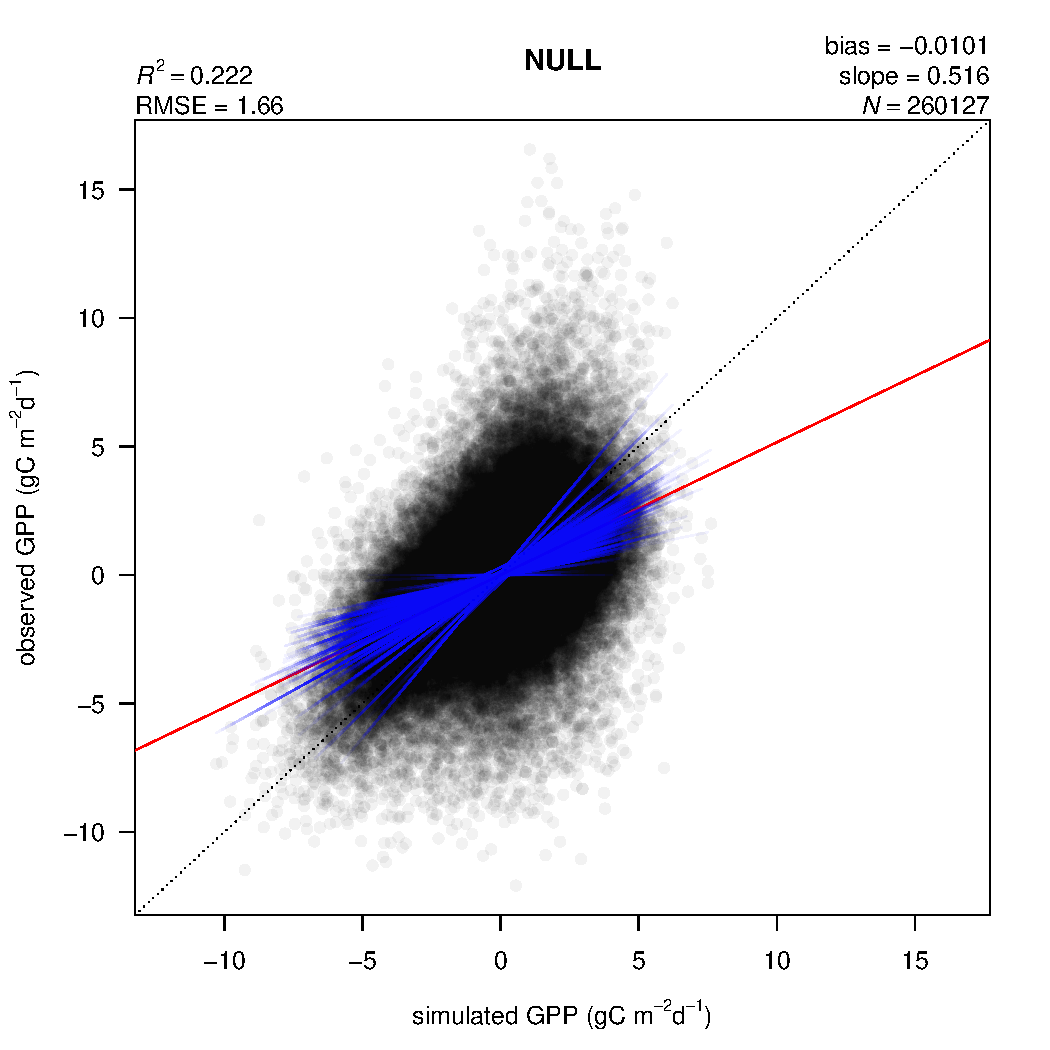
\includegraphics[width=0.4\textwidth]{fig/modobs_anomalies_daily_NULL.pdf}
%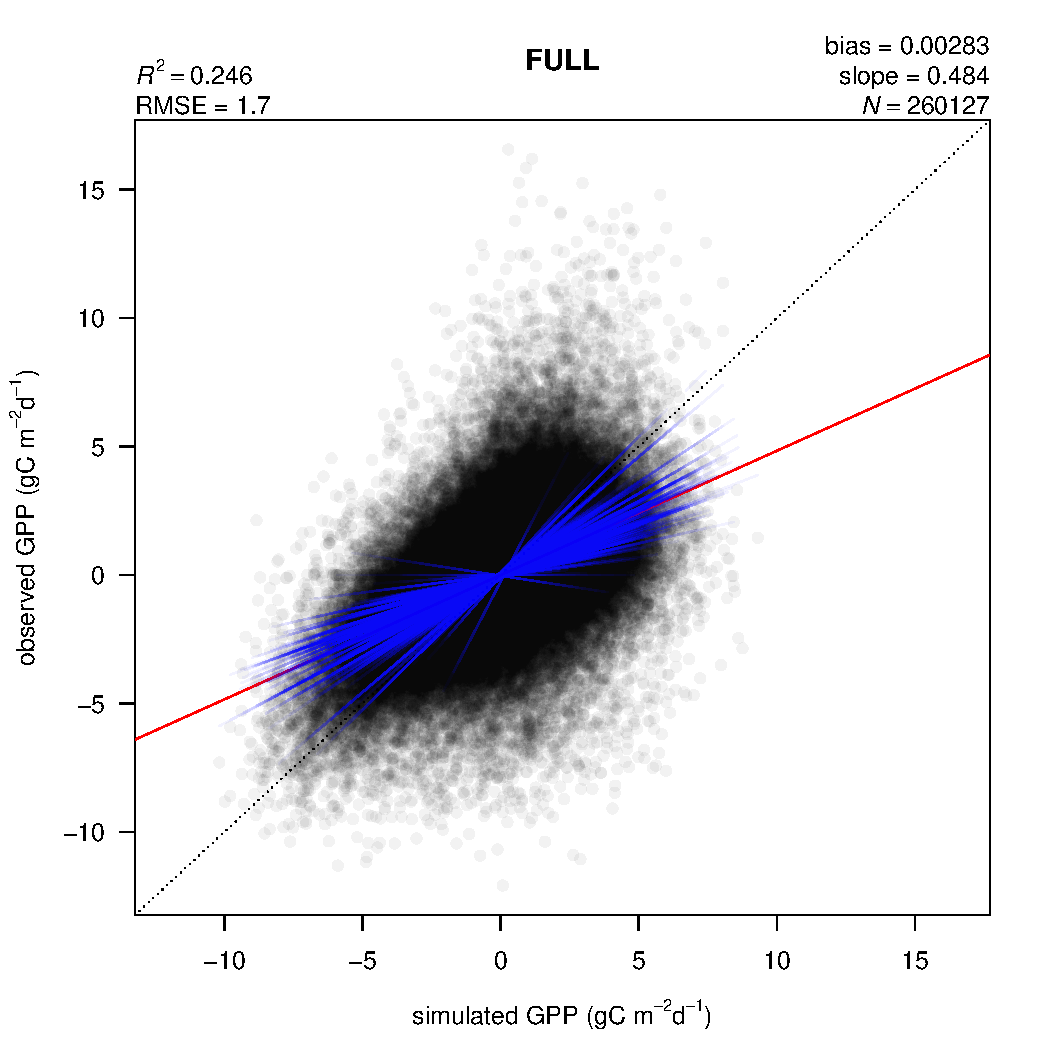
\includegraphics[width=0.4\textwidth]{fig/modobs_anomalies_daily_FULL.pdf}\\
%\includegraphics[width=0.4\textwidth]{fig/hist_anomalies_daily_NULL.pdf}
%\includegraphics[width=0.4\textwidth]{fig/hist_anomalies_daily_FULL.pdf}
    \caption{Daily anomalies from the mean seasonal cycle. Top row: The cloud of points illustrates daily anomalies from the mean seasonal cycle, blue lines are linear regressions for each site, and the red line is the linear regression of all data pooled. Bottom row: Histogram of daily anomalies from the mean seasonal cycle in the respective model and observations.}
    \label{fig:modobs_anomalies}
\end{figure}

\clearpage

\subsection{Greenness data}

Model predictions are highly sensitive to the greenness data used as model forcing. We investigated whether certain aspects of model-data disagreement (using standard splined MODIS FPAR data as forcing) can be resolved when alternative greenness forcing data is applied. As alternatives, we used MODIS EVI and a linearly interpolated version of MODIS FPAR. In particular, we investigated the following aspects of model-data disagreement:
\begin{itemize}
    \item Early season GPP overestimation in Dfb and Dfc north 
    \item Underestimation of GPP in mid-season in Cfb north
    \item Underestimation of peak-season GPP in Aw south
\end{itemize}

 \begin{figure}[!ht]
    \centering
\includegraphics[width=0.4\textwidth]{fig/meandoy_byzone_Dfb_north_greenness.pdf}
\includegraphics[width=0.4\textwidth]{fig/meandoy_byzone_Dfc_north_greenness.pdf}\\
\includegraphics[width=0.4\textwidth]{fig/meandoy_byzone_Cfb_north_greenness.pdf}
\includegraphics[width=0.4\textwidth]{fig/meandoy_byzone_Aw_south_greenness.pdf}
    \caption{Mean seasonal cycle for model setus with different greenness forcing data. Observations are given by the black line and grey band, representing the median and 33/66 \% quantiles of all data (multiple sites and years) pooled by climate zone. Coloured lines represent model setups, forced with different greenness data. The red band represents 33/66 \% quantiles for the model setup `FULL'. The annotation above each plot specifies the climate zone (see Tab. \ref{tab:kgclimate}), and $N$ given in the top right corner gives the number of sites within the respective climate zone for which data was used. Climate zones shown here are illustrative examples.}
    \label{fig:season_greenness}
\end{figure}

\begin{figure}[!ht]
    \centering
    \includegraphics[width=0.7\textwidth]{fig/modobs_spatial_annual_FULL.pdf}
    \includegraphics[width=0.7\textwidth]{fig/modobs_spatial_annual_EVI.pdf}
    \caption{Correlation of modelled and observed annual GPP for model setups using different greenness forcing data (MODIS FPAR MCD15A3H, splined in `FULL' and MODIS EVI MOD13Q1 in `EVI'). The red line and text are based on means across years by site and represents spatial (across-site) variations. Black lines and text are based on annual values, one line for each site. Lines represent linear regressions. $R^2$ and RMSE statistics for annual values (black text) are based on pooled data from all sites.}
    \label{fig:modobs_spatialannual_greenness}
\end{figure}

\clearpage

\subsection{GPP target data}

Are certain aspects of model-data disagreement related to uncertainty in the GPP flux decomposition? Above, we used NT data for calibration and evaluation. We additionally tested using DT and GePiSaT flux decomposition. Note that this evaluation is done only with a subset of the sites and data points from above, using only dates for which data is available in all three datasets. Therefore NT evaluations, repeated here, are not identical to the ones above. 
\begin{itemize}
    \item Early season GPP overestimation in Dfb and Dfc north 
    \item Peak-season GPP overestimation in Csa north
    \item Underestimation of peak-season GPP in Aw south
\end{itemize}

\begin{figure}[!ht]
    \centering
%\includegraphics[width=0.5\textwidth]{fig/modobs_xdaily_NT.pdf}
%\includegraphics[width=0.5\textwidth]{fig/modobs_xdaily_DT.pdf}
%\includegraphics[width=0.5\textwidth]{fig/modobs_xdaily_Ty.pdf}
    \caption{Correlation of observed and modelled GPP values of all sites pooled, mean over 10-day periods, determined from comparing respectively calibrated models to different observational GPP data (based on different flux decomposition methods, `DT' for the daytime method, `NT' for the nighttime method and `Ty' for the method by Davis et al. (xxx unpublished?))}
    \label{fig:modobs_10d_gppdata}
\end{figure}

\clearpage

\subsection{Functional relationships}

\begin{figure}[!ht]
\includegraphics[width=0.45\textwidth]{fig/functionalrel_gam_temp.pdf}
\includegraphics[width=0.45\textwidth]{fig/functionalrel_gam_vpd.pdf}
\includegraphics[width=0.45\textwidth]{fig/functionalrel_gam_soilm.pdf}
    \caption{Functional relationship of LUE in response to temperature, VPD, and soil moisture. Functional relationships in different observational data (`NT', `DT', `Ty') are determined by GAMs. `P-model, GAM' is determined from the model outputs for the same data points as `NT', `DT', and `Ty'. `P-model' is determined from applying the model directly. A more detailed description of the method is given in Section \ref{sec:gam}}
    \label{fig:functionalrel}
\end{figure}

\clearpage

\subsection{Drought response}

\begin{figure}[!ht]
    \centering
\includegraphics[width=0.8\textwidth]{fig/droughtresponse.pdf}
    \caption{}
    \label{fig:modobs_droughtresponse}
\end{figure}

\clearpage

% \subsubsection{VPD}

% Vapour pressure deficit ($D$) is calculated from vapour pressure (CRU) or specific humidity (WATCH-WFDEI) input data. In general, $D$ is the difference between actual and saturation vapour pressure:
% \begin{equation}
%     D = e_a - e_s
% \end{equation}
% We calculate saturation vapour pressure ($e_s$, in Pa) following Allen et al. (2005) as a function of temperature  as
% \begin{equation}
% e_s = 611 \; \exp \left( {\frac{17.27\;T_C}{T_C+237.3}} \right)
% \end{equation}
% $T_C$ is the temperature expressed in units of degrees Celsius. Note that Allen et al. (2005) use 6.108 instead of 6.11. The Python implementation uses daily maximum and daily minimum temperature, which is equivalent to above formulation with $T=(T_{\text{min}}+T_{\text{max}})/2$. $e_a$ is provided by CRU as an input dataset. WATCH-WFDEI provides specific humidity data ($q$), which can be converted to the mass mixing ratio of water vapor to dry air ($w$) (dimensionless) by
% \begin{equation}
%     w = \frac{q}{1-q}
% \end{equation}
% and finally to actual vapour pressure by
% \begin{equation}
%     e_a = P \frac{w R_v}{R_d + w R_v}
% \end{equation}
% where $P$ is the atmospheric pressure (Pa), $R_v$ is the specific gas constant for water vapour and $R_d$ is the specific gas constant for dry air. The specific gas constants are calculated from the universal gas constant $R$ and the molecular mass $M$ as $R_{\text{specific}}=R/M$. ($R$ is 8.3143 J mol$^{-1}$ K$^{-1}$. The molecular mass of dry air is $M_d=$ 28.963 g mol$^{-1}$ and the molecular mass of water vapor is $M_v=$ 18.02 g mol$^{-1}$.) Atmospheric pressure is assumed to be at standard conditions (101325 Pa) corrected for local elevation (barometric formula adopted from SPLASH, Eq. 20 in Davis et al., 2017).




% \begin{table}
% \centering
% \begin{tabular}{ p{1.2cm} p{2.5cm} p{2.5cm} p{4cm} l }
% \multicolumn{5}{l}{\textbf{ WATCH-WFDEI }} \\
% \hline
% \textbf{symbol} & \textbf{variable name} & \textbf{file name} & \textbf{variable description} & \textbf{units} \\
% \hline
% $T$ & \texttt{Tair} & \texttt{Tair\_WFDEI} & 2 m instantaneous air temperature & K \\
% $P_{\text{rain}}$    & \texttt{Rainf}  & \texttt{Rainf\_WFDEI\_CRU} & Rainfall rate, bias corrected with CRU TS3.101 data (TS3.21 for 2010-2012) and gauge ``catch corrected'' (average over previous 3 hrs) & kg m$^{-2}$ s$^{-1}$ \\  
% $P_{\text{snow}}$    & \texttt{Snowf} & \texttt{Snowf\_WFDEI\_CRU} & Snowfall rate, bias corrected with CRU TS3.101 data (TS3.21 for 2010-2012) and gauge ``catch corrected'' (average over previous 3 hrs)  & kg m$^{-2}$ s$^{-1}$ \\  
% $R_{\text{SW}}$    & \texttt{SWdown} & \texttt{SWdown\_WFDEI} & Short-wave downwards surface radiation flux (average over previous 3 hours) & W m$^{-2}$ \\  
% $q$    & \texttt{Qair} & \texttt{Qair\_WFDEI} & 2 m instantaneous specific humidity & kg kg$^{-1}$ \\  
% $p$    & \texttt{PSurf} & \texttt{PSurf\_WFDEI} & Instantaneous surface pressure & Pa \\ 
% \hline
% \end{tabular}
% \caption{Variables used from WATCH-WFDEI meteorological data.}
% \label{tab:meteovars}
% \end{table}


\subsection{Green vegetation cover}


\section{Evaluation against FLUXNET data}

Several performance metrics are calculated for different features of GPP variability. The performance metrics are:
\begin{itemize}
    \item R$^2$
    \item RMSE
    \item slope (of regression observed over modelled)
    \item bias
\end{itemize}

The features of variability in GPP, for which model-observation agreement is calculated, are:
\begin{itemize}
    \item mean annual values (giving "spatial" correlation)
    \item annual anomalies from mean across years
    \item daily values, absolute
    \item mean across X-day periods, absolute
    \item mean seasonal cycle (mean by day of year)
    \item daily anomalies from mean seasonal cycle
\end{itemize}

\clearpage

\subsection{Spatial correlation}

\begin{figure}[!ht]
    \centering
    %\includegraphics[width=0.8\textwidth]{fig/modobs_spatial.pdf}
    \caption{Correlation of observed vs. modelled mean annual GPP by site.}
    \label{fig:modobs_spatial}
\end{figure}

\clearpage


\subsection{Annual GPP anomalies}

\begin{figure}[!ht]
    \centering
    %\includegraphics[width=0.8\textwidth]{fig/modobs_anomalies_annual.pdf}
    \caption{Correlation of observed vs. modelled annual GPP anomalies from mean across multiple years.}
    \label{fig:modobs_iav}
\end{figure}

\clearpage


\subsection{Combined spatial/annual}

\begin{figure}[!ht]
    \centering
    %\includegraphics[width=0.8\textwidth]{fig/modobs_spatial_annual.pdf}
    \caption{Spatial and annual correlation of observed over modelled annual GPP by site.}
    \label{fig:modobs_spatialannual}
\end{figure}

\clearpage


\section{Sites and data processing}

\begin{longtable}{lrrlllrl}
  \hline
 Site & Lon. & Lat. & Period & Veg. & Clim. & N & Reference \\ 
  \hline
 AR-SLu & -66.46 & -33.46 & 2009-2011 & MF & Bwk & 430 & \cite{AR-SLu} \\ 
 AR-Vir & -56.19 & -28.24 & 2009-2012 & ENF & Csb & 585 & \cite{AR-Vir} \\ 
 AT-Neu & 11.32 & 47.12 & 2002-2012 & GRA & Dfc & 3172 & \cite{AT-Neu} \\ 
 AU-Ade & 131.12 & -13.08 & 2007-2009 & WSA & Aw & 528 & \cite{AU-Ade} \\ 
 AU-ASM & 133.25 & -22.28 & 2010-2013 & ENF & BSh & 863 & \cite{AU-ASM} \\ 
 AU-Cpr & 140.59 & -34.00 & 2010-2014 & SAV & BSk & 1346 & \cite{AU-Cpr} \\ 
 AU-Cum & 150.72 & -33.61 & 2012-2014 & EBF & Cfa & 727 & \cite{AU-Cum} \\ 
 AU-DaP & 131.32 & -14.06 & 2007-2013 & GRA & Aw & 1377 & \cite{AU-DaP} \\ 
 AU-DaS & 131.39 & -14.16 & 2008-2014 & SAV & Aw & 2148 & \cite{AU-DaS} \\ 
 AU-Dry & 132.37 & -15.26 & 2008-2014 & SAV & Aw & 1579 & \cite{AU-Dry} \\ 
 AU-Emr & 148.47 & -23.86 & 2011-2013 & GRA & Bwk & 674 & \cite{AU-Emr} \\ 
 AU-Fog & 131.31 & -12.55 & 2006-2008 & WET & Aw & 866 & \cite{AU-Fog} \\ 
 AU-Gin & 115.71 & -31.38 & 2011-2014 & WSA & Cwb & 935 & \cite{AU-Gin} \\ 
 AU-GWW & 120.65 & -30.19 & 2013-2014 & SAV & Bwk & 646 & \cite{AU-GWW} \\ 
 AU-How & 131.15 & -12.49 & 2001-2014 & WSA & Aw &  & \cite{AU-How} \\ 
 AU-Lox & 140.66 & -34.47 & 2008-2009 & DBF & Bsh & 271 & \cite{AU-Lox} \\ 
 AU-RDF & 132.48 & -14.56 & 2011-2013 & WSA & Bwh & 424 & \cite{AU-RDF} \\ 
 AU-Rig & 145.58 & -36.65 & 2011-2014 & GRA & Cfb & 1116 & \cite{AU-Rig} \\ 
 AU-Rob & 145.63 & -17.12 & 2014-2014 & EBF & Csb & 314 & \cite{AU-Rob} \\ 
 AU-Stp & 133.35 & -17.15 & 2008-2014 & GRA & BSh & 1314 & \cite{AU-Stp} \\ 
 AU-TTE & 133.64 & -22.29 & 2012-2013 & OSH & BWh &  89 & \cite{AU-TTE} \\ 
 AU-Tum & 148.15 & -35.66 & 2001-2014 & EBF & Cfb & 4176 & \cite{AU-Tum} \\ 
 AU-Wac & 145.19 & -37.43 & 2005-2008 & EBF & Cfb & 968 & \cite{AU-Wac} \\ 
 AU-Whr & 145.03 & -36.67 & 2011-2014 & EBF & Cfb & 1062 & \cite{AU-Whr} \\ 
 AU-Wom & 144.09 & -37.42 & 2010-2012 & EBF & Cfb & 897 & \cite{AU-Wom} \\ 
 AU-Ync & 146.29 & -34.99 & 2012-2014 & GRA & BSk & 336 & \cite{AU-Ync} \\ 
 BE-Bra & 4.52 & 51.31 & 1996-2014 & MF & Cfb & 4458 & \cite{BE-Bra} \\ 
 BE-Lon & 4.75 & 50.55 & 2004-2014 & CRO & Cfb & 2834 & \cite{BE-Lon} \\ 
 BE-Vie & 6.00 & 50.31 & 1996-2014 & MF & Cfb & 5556 & \cite{BE-Vie} \\ 
 BR-Sa3 & -54.97 & -3.02 & 2000-2004 & EBF & Am & 1122 & \cite{BR-Sa3} \\ 
 CA-Man & -98.48 & 55.88 & 1994-2008 & ENF & Dfc & 2435 & \cite{CA-Man} \\ 
 CA-NS1 & -98.48 & 55.88 & 2001-2005 & ENF & Dfc & 763 & \cite{CA-NS1} \\ 
 CA-NS2 & -98.52 & 55.91 & 2001-2005 & ENF & Dfc & 859 & \cite{CA-NS2} \\ 
 CA-NS3 & -98.38 & 55.91 & 2001-2005 & ENF & Dfc & 1062 & \cite{CA-NS3} \\ 
 CA-NS4 & -98.38 & 55.91 & 2002-2005 & ENF & Dfc & 601 & \cite{CA-NS4} \\ 
 CA-NS5 & -98.48 & 55.86 & 2001-2005 & ENF & Dfc & 903 & \cite{CA-NS5} \\ 
 CA-NS6 & -98.96 & 55.92 & 2001-2005 & OSH & Dfc & 904 & \cite{CA-NS6} \\ 
 CA-NS7 & -99.95 & 56.64 & 2002-2005 & OSH & Dfc & 693 & \cite{CA-NS7} \\ 
 CA-Qfo & -74.34 & 49.69 & 2003-2010 & ENF & Dfc & 1795 & \cite{CA-Qfo} \\ 
 CA-SF1 & -105.82 & 54.48 & 2003-2006 & ENF & Dfc & 513 & \cite{CA-SF1} \\ 
 CA-SF2 & -105.88 & 54.25 & 2001-2005 & ENF & Dfc & 664 & \cite{CA-SF2} \\ 
 CA-SF3 & -106.01 & 54.09 & 2001-2006 & OSH & Dfc & 634 & \cite{CA-SF3} \\ 
 CH-Cha & 8.41 & 47.21 & 2005-2014 & GRA & Cfb & 2872 & \cite{CH-Cha} \\ 
 CH-Dav & 9.86 & 46.82 & 1997-2014 & ENF & ET & 5293 & \cite{CH-Dav} \\ 
 CH-Fru & 8.54 & 47.12 & 2005-2014 & GRA & Cfb & 2527 & \cite{CH-Fru} \\ 
 CH-Lae & 8.37 & 47.48 & 2004-2014 & MF & Cfb & 3144 & \cite{CH-Lae} \\ 
 CH-Oe1 & 7.73 & 47.29 & 2002-2008 & GRA & Cfb & 2083 & \cite{CH-Oe1} \\ 
 CH-Oe2 & 7.73 & 47.29 & 2004-2014 & CRO & Cfb & 2990 & \cite{CH-Oe2} \\ 
 CN-Cha & 128.10 & 42.40 & 2003-2005 & MF & Dwb & 804 & \cite{CN-Cha} \\ 
 CN-Cng & 123.51 & 44.59 & 2007-2010 & GRA & Bsh & 1026 & \cite{CN-Cng} \\ 
 CN-Dan & 91.07 & 30.50 & 2004-2005 & GRA & ET & 619 & \cite{CN-Dan} \\ 
 CN-Din & 112.54 & 23.17 & 2003-2005 & EBF & Cfa & 894 & \cite{CN-Din} \\ 
 CN-Du2 & 116.28 & 42.05 & 2006-2008 & GRA & Dwb & 520 & \cite{CN-Du2} \\ 
 CN-Ha2 & 101.33 & 37.61 & 2003-2005 & WET & ET & 886 & \cite{CN-Ha2} \\ 
 CN-HaM & 101.18 & 37.37 & 2002-2004 & GRA &  & 664 & \cite{CN-HaM} \\ 
 CN-Qia & 115.06 & 26.74 & 2003-2005 & ENF & Cfa & 987 & \cite{CN-Qia} \\ 
 CN-Sw2 & 111.90 & 41.79 & 2010-2012 & GRA & Bsh & 202 & \cite{CN-Sw2} \\ 
 CZ-BK1 & 18.54 & 49.50 & 2004-2008 & ENF & Dfb & 1051 & \cite{CZ-BK1} \\ 
 CZ-BK2 & 18.54 & 49.49 & 2004-2006 & GRA & Dfb & 156 & \cite{CZ-BK2} \\ 
 CZ-wet & 14.77 & 49.02 & 2006-2014 & WET & Cfb & 2592 & \cite{CZ-wet} \\ 
 DE-Akm & 13.68 & 53.87 & 2009-2014 & WET & Cfb &  & \cite{DE-Akm} \\ 
 DE-Geb & 10.91 & 51.10 & 2001-2014 & CRO & Cfb & 3454 & \cite{DE-Geb} \\ 
 DE-Gri & 13.51 & 50.95 & 2004-2014 & GRA & Cfb & 3349 & \cite{DE-Gri} \\ 
 DE-Hai & 10.45 & 51.08 & 2000-2012 & DBF & Cfb & 3436 & \cite{DE-Hai} \\ 
 DE-Kli & 13.52 & 50.89 & 2004-2014 & CRO & Cfb &  & \cite{DE-Kli} \\ 
 DE-Lkb & 13.30 & 49.10 & 2009-2013 & ENF & Cfb & 846 & \cite{DE-Lkb} \\ 
 DE-Obe & 13.72 & 50.78 & 2008-2014 & ENF & Cfb & 1992 & \cite{DE-Obe} \\ 
 DE-RuR & 6.30 & 50.62 & 2011-2014 & GRA & Cfb & 1178 & \cite{DE-RuR} \\ 
 DE-RuS & 6.45 & 50.87 & 2011-2014 & CRO & Cfb &  & \cite{DE-RuS} \\ 
 DE-Seh & 6.45 & 50.87 & 2007-2010 & CRO & Cfb & 1026 & \cite{DE-Seh} \\ 
 DE-SfN & 11.33 & 47.81 & 2012-2014 & WET & Cfb & 737 & \cite{DE-SfN} \\ 
 DE-Spw & 14.03 & 51.89 & 2010-2014 & WET & Cfb & 1323 & \cite{DE-Spw} \\ 
 DE-Tha & 13.57 & 50.96 & 1996-2014 & ENF & Cfb & 5964 & \cite{DE-Tha} \\ 
 DK-Fou & 9.59 & 56.48 & 2005-2005 & CRO & Cfb & 212 & \cite{DK-Fou} \\ 
 DK-NuF & -51.39 & 64.13 & 2008-2014 & WET & ET & 869 & \cite{DK-NuF} \\ 
 DK-Sor & 11.64 & 55.49 & 1996-2014 & DBF & Cfb & 5514 & \cite{DK-Sor} \\ 
 DK-ZaF & -20.55 & 74.48 & 2008-2011 & WET & ET & 328 & \cite{DK-ZaF} \\ 
 DK-ZaH & -20.55 & 74.47 & 2000-2014 & GRA & ET & 1648 & \cite{DK-ZaH} \\ 
 ES-LgS & -2.97 & 37.10 & 2007-2009 & OSH & Cwc & 766 & \cite{ES-LgS} \\ 
 ES-Ln2 & -3.48 & 36.97 & 2009-2009 & OSH & Cwc &  61 & \cite{ES-Ln2} \\ 
 FI-Hyy & 24.30 & 61.85 & 1996-2014 & ENF & Dfc & 5204 & \cite{FI-Hyy} \\ 
 FI-Jok & 23.51 & 60.90 & 2000-2003 & CRO & Dfc & 595 & \cite{FI-Jok} \\ 
 FI-Lom & 24.21 & 68.00 & 2007-2009 & WET & Dfc & 430 & \cite{FI-Lom} \\ 
 FI-Sod & 26.64 & 67.36 & 2001-2014 & ENF & Dfc & 2634 & \cite{FI-Sod} \\ 
 FR-Fon & 2.78 & 48.48 & 2005-2014 & DBF & Cfb & 2821 & \cite{FR-Fon} \\ 
 FR-Gri & 1.95 & 48.84 & 2004-2013 & CRO & Cfb &  & \cite{FR-Gri} \\ 
 FR-LBr & -0.77 & 44.72 & 1996-2008 & ENF & Cfb & 3527 & \cite{FR-LBr} \\ 
 FR-Pue & 3.60 & 43.74 & 2000-2014 & EBF & Cwb & 4650 & \cite{FR-Pue} \\ 
 GF-Guy & -52.92 & 5.28 & 2004-2014 & EBF & Am & 3583 & \cite{GF-Guy} \\ 
 IT-BCi & 14.96 & 40.52 & 2004-2014 & CRO & Cwb &  & \cite{IT-BCi} \\ 
 IT-CA1 & 12.03 & 42.38 & 2011-2014 & DBF & Cwb & 991 & \cite{IT-CA1} \\ 
 IT-CA2 & 12.03 & 42.38 & 2011-2014 & CRO & Cwb & 959 & \cite{IT-CA2} \\ 
 IT-CA3 & 12.02 & 42.38 & 2011-2014 & DBF & Cwb & 813 & \cite{IT-CA3} \\ 
 IT-Col & 13.59 & 41.85 & 1996-2014 & DBF & Cfa & 3276 & \cite{IT-Col} \\ 
 IT-Cp2 & 12.36 & 41.70 & 2012-2014 & EBF & Cwb & 756 & \cite{IT-Cp2} \\ 
 IT-Cpz & 12.38 & 41.71 & 1997-2009 & EBF & Cwb & 2536 & \cite{IT-Cpz} \\ 
 IT-Isp & 8.63 & 45.81 & 2013-2014 & DBF & Cfb & 557 & \cite{IT-Isp} \\ 
 IT-La2 & 11.29 & 45.95 & 2000-2002 & ENF & Cfb & 470 & \cite{IT-La2} \\ 
 IT-Lav & 11.28 & 45.96 & 2003-2014 & ENF & Cfb & 3799 & \cite{IT-Lav} \\ 
 IT-MBo & 11.05 & 46.01 & 2003-2013 & GRA & Dfb & 3203 & \cite{IT-MBo} \\ 
 IT-Noe & 8.15 & 40.61 & 2004-2014 & CSH & Cwb & 3013 & \cite{IT-Noe} \\ 
 IT-PT1 & 9.06 & 45.20 & 2002-2004 & DBF & Cfa & 813 & \cite{IT-PT1} \\ 
 IT-Ren & 11.43 & 46.59 & 1998-2013 & ENF & Dfc & 3180 & \cite{IT-Ren} \\ 
 IT-Ro1 & 11.93 & 42.41 & 2000-2008 & DBF & Cwb &  & \cite{IT-Ro1} \\ 
 IT-Ro2 & 11.92 & 42.39 & 2002-2012 & DBF & Cwb & 2641 & \cite{IT-Ro2} \\ 
 IT-SR2 & 10.29 & 43.73 & 2013-2014 & ENF & Cwb & 658 & \cite{IT-SR2} \\ 
 IT-SRo & 10.28 & 43.73 & 1999-2012 & ENF & Cwb & 4021 & \cite{IT-SRo} \\ 
 IT-Tor & 7.58 & 45.84 & 2008-2014 & GRA & Dfc & 1351 & \cite{IT-Tor} \\ 
 JP-MBF & 142.32 & 44.39 & 2003-2005 & DBF & Dfb & 459 & \cite{JP-MBF} \\ 
 JP-SMF & 137.08 & 35.26 & 2002-2006 & MF & Cfa & 1272 & \cite{JP-SMF} \\ 
 NL-Hor & 5.07 & 52.24 & 2004-2011 & GRA & Cfb & 2113 & \cite{NL-Hor} \\ 
 NL-Loo & 5.74 & 52.17 & 1996-2013 & ENF & Cfb & 5417 & \cite{NL-Loo} \\ 
 NO-Adv & 15.92 & 78.19 & 2011-2014 & WET & ET &  90 & \cite{NO-Adv} \\ 
 NO-Blv & 11.83 & 78.92 & 2008-2009 & SNO & ET &  60 & \cite{NO-Blv} \\ 
 RU-Che & 161.34 & 68.61 & 2002-2005 & WET & Dfc & 277 & \cite{RU-Che} \\ 
 RU-Cok & 147.49 & 70.83 & 2003-2014 & OSH & Dfc & 962 & \cite{RU-Cok} \\ 
 RU-Fyo & 32.92 & 56.46 & 1998-2014 & ENF & Dfb & 4397 & \cite{RU-Fyo} \\ 
 RU-Ha1 & 90.00 & 54.73 & 2002-2004 & GRA & Dfc & 516 & \cite{RU-Ha1} \\ 
 SD-Dem & 30.48 & 13.28 & 2005-2009 & SAV & BWh & 735 & \cite{SD-Dem} \\ 
 SN-Dhr & -15.43 & 15.40 & 2010-2013 & SAV & BWh & 631 & \cite{SN-Dhr} \\ 
 US-AR1 & -99.42 & 36.43 & 2009-2012 & GRA & Cfa & 925 & \cite{US-AR1} \\ 
 US-AR2 & -99.60 & 36.64 & 2009-2012 & GRA & Cfa & 810 & \cite{US-AR2} \\ 
 US-ARb & -98.04 & 35.55 & 2005-2006 & GRA & Cfa & 408 & \cite{US-ARb} \\ 
 US-ARc & -98.04 & 35.55 & 2005-2006 & GRA & Cfa & 478 & \cite{US-ARc} \\ 
 US-ARM & -97.49 & 36.61 & 2003-2012 & CRO & Cfa & 2306 & \cite{US-ARM} \\ 
 US-Blo & -120.63 & 38.90 & 1997-2007 & ENF & Cwc & 2227 & \cite{US-Blo} \\ 
 US-Cop & -109.39 & 38.09 & 2001-2007 & GRA & BSk & 933 & \cite{US-Cop} \\ 
 US-GBT & -106.24 & 41.37 & 1999-2006 & ENF & Dfc & 533 & \cite{US-GBT} \\ 
 US-GLE & -106.24 & 41.37 & 2004-2014 & ENF & Dfb & 2146 & \cite{US-GLE} \\ 
 US-Ha1 & -72.17 & 42.54 & 1991-2012 & DBF & Dfb & 4810 & \cite{US-Ha1} \\ 
 US-KS2 & -80.67 & 28.61 & 2003-2006 & CSH & Cfa & 1255 & \cite{US-KS2} \\ 
 US-Los & -89.98 & 46.08 & 2000-2014 & WET & Dfb & 2040 & \cite{US-Los} \\ 
 US-Me1 & -121.50 & 44.58 & 2004-2005 & ENF & Cwc & 260 & \cite{US-Me1} \\ 
 US-Me2 & -121.56 & 44.45 & 2002-2014 & ENF & Cwc & 3399 & \cite{US-Me2} \\ 
 US-Me6 & -121.61 & 44.32 & 2010-2014 & ENF & Cwc & 1243 & \cite{US-Me6} \\ 
 US-MMS & -86.41 & 39.32 & 1999-2014 & DBF & Cfa & 3610 & \cite{US-MMS} \\ 
 US-Myb & -121.77 & 38.05 & 2010-2014 & WET & Cwb & 1111 & \cite{US-Myb} \\ 
 US-Ne1 & -96.48 & 41.17 & 2001-2013 & CRO & Dfa &  & \cite{US-Ne1} \\ 
 US-Ne2 & -96.47 & 41.16 & 2001-2013 & CRO & Dfa &  & \cite{US-Ne2} \\ 
 US-Ne3 & -96.44 & 41.18 & 2001-2013 & CRO & Dfa &  & \cite{US-Ne3} \\ 
 US-NR1 & -105.55 & 40.03 & 1998-2014 & ENF & Dfc & 4205 & \cite{US-NR1} \\ 
 US-ORv & -83.02 & 40.02 & 2011-2011 & WET & Dfa &  & \cite{US-ORv} \\ 
 US-PFa & -90.27 & 45.95 & 1995-2014 & MF & Dfb & 4590 & \cite{US-PFa} \\ 
 US-Prr & -147.49 & 65.12 & 2010-2013 & ENF & Dfc & 515 & \cite{US-Prr} \\ 
 US-SRG & -110.83 & 31.79 & 2008-2014 & GRA & BSk & 1874 & \cite{US-SRG} \\ 
 US-SRM & -110.87 & 31.82 & 2004-2014 & WSA & BSk & 2759 & \cite{US-SRM} \\ 
 US-Syv & -89.35 & 46.24 & 2001-2014 & MF & Dfb & 1977 & \cite{US-Syv} \\ 
 US-Ton & -120.97 & 38.43 & 2001-2014 & WSA & Cwb & 3981 & \cite{US-Ton} \\ 
 US-Tw1 & -121.65 & 38.11 & 2012-2014 & WET & Cwb & 554 & \cite{US-Tw1} \\ 
 US-Tw2 & -121.64 & 38.10 & 2012-2013 & CRO & Cwb & 263 & \cite{US-Tw2} \\ 
 US-Tw3 & -121.65 & 38.12 & 2013-2014 & CRO & Cwb & 419 & \cite{US-Tw3} \\ 
 US-Tw4 & -121.64 & 38.10 & 2013-2014 & WET & Cwb & 321 & \cite{US-Tw4} \\ 
 US-Twt & -121.65 & 38.11 & 2009-2014 & CRO & Cwb & 1421 & \cite{US-Twt} \\ 
 US-UMB & -84.71 & 45.56 & 2000-2014 & DBF & Dfb & 3970 & \cite{US-UMB} \\ 
 US-UMd & -84.70 & 45.56 & 2007-2014 & DBF & Dfb & 2034 & \cite{US-UMd} \\ 
 US-Var & -120.95 & 38.41 & 2000-2014 & GRA & Cwb & 2931 & \cite{US-Var} \\ 
 US-WCr & -90.08 & 45.81 & 1999-2014 & DBF & Dfb & 2485 & \cite{US-WCr} \\ 
 US-Whs & -110.05 & 31.74 & 2007-2014 & OSH & BSk & 1452 & \cite{US-Whs} \\ 
 US-Wi0 & -91.08 & 46.62 & 2002-2002 & ENF & Dfb & 175 & \cite{US-Wi0} \\ 
 US-Wi3 & -91.10 & 46.63 & 2002-2004 & DBF & Dfb & 353 & \cite{US-Wi3} \\ 
 US-Wi4 & -91.17 & 46.74 & 2002-2005 & ENF & Dfb & 568 & \cite{US-Wi4} \\ 
 US-Wi6 & -91.30 & 46.62 & 2002-2003 & OSH & Dfb & 175 & \cite{US-Wi6} \\ 
 US-Wi9 & -91.08 & 46.62 & 2004-2005 & ENF & Dfb & 290 & \cite{US-Wi9} \\ 
 US-Wkg & -109.94 & 31.74 & 2004-2014 & GRA & BSk & 2373 & \cite{US-Wkg} \\ 
 ZA-Kru & 31.50 & -25.02 & 2000-2010 & SAV & BSh & 1890 & \cite{ZA-Kru} \\ 
 ZM-Mon & 23.25 & -15.44 & 2000-2009 & DBF & Aw & 625 & \cite{ZM-Mon} \\ 
  \hline
\caption{Sites used for evaluation. Lon. is longitude, negative values indicate west longitude; Lat. is latitude, positive values indicate north latitude; Veg. is vegetation type: deciduous broadleaf forest (DBF); evergreen broadleaf forest (EBF); evergreen needleleaf forest (ENF); grassland (GRA); mixed deciduous and evergreen needleleaf forest (MF); savanna ecosystem (SAV); shrub ecosystem (SHR); wetland (WET).} 
\end{longtable}

%% \\\\\\\\\\\\\\\\\\\\\\\\\\\\\\\\\\\\\\\\\\\\\\\\\\\\\\\\\\\\\\\\\\\\\\\\ %%
%% PART 3.2.2 -- RELATIVE VISCOSITY OF WATER
%% //////////////////////////////////////////////////////////////////////// %%
\subsection{Relative Viscosity of Water}
\label{sec:eta}
The viscosity of water at a given temperature and pressure, $\eta$, may be calculated based on the methodology of \cite{huber09}. 
The relative viscosity of water with respect to its value at 25 ${}^\circ$C, $\eta^\ast$, is calculated by the following ratio:
%% ---------------------------------------------------------------%%
%% eq:ns | Relative viscosity of water
%% ---------------------------------------------------------------%%
\nomenclature{$\eta^\ast$}{relative viscosity of water [unitless]}%
\begin{equation}
\label{eq:ns}
    \eta^\ast = \frac{\eta}{\eta_{25}}
\end{equation}

\noindent where:\\
\indent $\eta$ = viscosity of water at a given temperature and pressure [Pa s];\\
\indent $\eta_{25}$ = viscosity at 25 ${}^\circ$C and standard pressure [8.90$\times 10^{-4}$ Pa s].\\

%% \\\\\\\\\\\\\\\\\\\\\\\\\\\\\\\\\\\\\\\\\\\\\\\\\\\\\\\\\\\\\\\\\\\\\\\\ %%
%% PART 3.2.3 -- AMBIENT PARTIAL PRESSURE OF CO2
%% //////////////////////////////////////////////////////////////////////// %%
\subsection{Ambient Partial Pressure of CO$_2$}
\label{sec:ca}
The partial pressure of CO$_2$, $c_a$, is calculated based on the observed annual atmospheric CO$_2$ concentration (see \S \ref{sec:gepnoaa}). 
The conversion can be done knowing the total atmospheric pressure, $P_{atm}$, and using Dalton's Law of Partial Pressure:
%% ---------------------------------------------------------------%%
%% eq:pp | Partial Pressure Convertion
%% ---------------------------------------------------------------%%
\begin{equation}
\label{eq:pp}
    p_x = 1\times 10^{-6}\; ppm_x\; P_{atm}
\end{equation}

\noindent where:\\
\indent $p_x$ = partial pressure of gas \textit{x} [Pa];\\
\indent $ppm_x$ = parts-per-million concentration of gas \textit{x} [ppm];\\
\indent $P_{atm}$ = total atmospheric pressure [Pa].\\

\noindent For instances when $P_{atm}$ is unknown, the elevation-dependent atmospheric pressure may be computed using the Barometric Formula, assuming a linear decrease in temperature with height within the troposphere and a mean adiabatic lapse rate \parencite{berberan97}:
%% ---------------------------------------------------------------%%
%% eq:pz | Atmospheric pressure as a function of elevation
%% ---------------------------------------------------------------%%
\nomenclature{$P_{atm}$}{total atmospheric pressure [Pa]}%
\begin{equation}
\label{eq:pz}
    P_{atm}\left( z \right) = P_{\circ} \left( 
    	1 - \frac{L\; z}{T_{\circ}} 
    \right)^{g\; M_a\; \left(R_u\; L\right)^{-1}}
\end{equation}

\noindent where:\\
\indent $z$ = altitude above mean sea level [m];\\
\indent $g$ = standard gravity [9.80665 m s$^{-2}$];\\
\indent $P_{\circ}$ = base atmospheric pressure [101325 Pa];\\
\indent $L$ = mean adiabatic lapse rate [0.0065 K m$^{-2}$];\\
\indent $T_{\circ}$ = base temperature [288.15 K];\\
\indent $M_a$ = molecular weight for dry air [0.028963 kg mol$^{-1}$];\\
\indent $R_u$ = universal gas constant [8.3145 J mol$^{-1}$ K$^{-1}$].\\

%% \\\\\\\\\\\\\\\\\\\\\\\\\\\\\\\\\\\\\\\\\\\\\\\\\\\\\\\\\\\\\\\\\\\\\\\\ %%
%% PART 3.2.4 -- VAPOR PRESSURE DEFICIT
%% //////////////////////////////////////////////////////////////////////// %%
\subsection{Vapor Pressure Deficit}
\label{sec:d}
The vapor pressure deficit, $D$, is based on the unit conversion of the observed VPD (see \S \ref{sec:gepvpd}) from kPa to Pa.

%% \\\\\\\\\\\\\\\\\\\\\\\\\\\\\\\\\\\\\\\\\\\\\\\\\\\\\\\
%% PHOTORESPIRATORY COMPENSATION POINT
%% ///////////////////////////////////////////////////////
\subsection{Photorespiratory Compensation Point}
\label{sec:gs}
The photorespiratory compensation point, $\Gamma^\ast$, is given by its value at standard temperature and atmospheric pressure $\Gamma^\ast_{25, p_0} = $ following \cite{bernacchi01xxx}, modified by temperature following an Arrhenius-type temperature response function $f_{\text{Arrh}}(T)$ with an activation energy of $\Delta H_a$, and corrected for atmospheric pressure. Values for parameters $\Gamma^\ast_{25, p_0}$, and $\Delta H_a$ are fixed and given in Tab. \ref{tab:params_fixed}.

\begin{equation}
\label{eq:gammastar}
    \Gamma^\ast (T, z) = \Gamma^\ast_{25, p_0} \; f_{\text{Arrh}}(T) \; \frac{p(z)}{p(z_0)}
\end{equation}


\begin{equation}
\label{eq:gsbasic}
    \Gamma^\ast = \frac{O\: K_c\: V_\text{o,max}}
                        {2\: K_o\: V_\text{c,max}}
\end{equation}

\noindent where:\\
\indent $O$ = partial pressure of atmospheric O$_2$, [Pa];\\
\indent $K_c$ = Michaelis-Menten constant for carboxylation [Pa];\\
\indent $K_o$ = Michaelis-Menten constant for oxygenation [Pa];\\
\indent $V_\text{c,max}$ = maximum rate of carboxylation [$\mu$mol~m$^{-2}$~s$^{-1}$];\\
\indent $V_\text{o,max}$ = maximum rate of oxygenation [$\mu$mol~m$^{-2}$~s$^{-1}$].\\

\noindent The temperature-dependency of $\Gamma^\ast$ is derived from the temperature dependencies of $K_c$, $K_o$, $V_\text{c,max}$, and $V_\text{o,max}$, which have been empirically solved by \cite{bernacchi01}. 
Substituting the temperature-dependency equations for each term in Eq. \ref{eq:gsbasic}, results in the following expression:
%% ---------------------------------------------------------------%%
%% eq:gst | Temperature dependency of Gamma*
%% ---------------------------------------------------------------%%
\begin{equation}
\label{eq:gst}
    \Gamma^\ast = \exp \left(7.472 - \frac{\Delta H_a}{R_u\: T_k}\right) \frac{O}{2}
\end{equation}

\noindent where:\\
\indent $\Delta H_a$ = activation energy for $\Gamma^\ast$ [37$\,$830 J mol$^{-1}$];\\
\indent $R_u$ = universal gas constant [8.3145 J mol$^{-1}$ K$^{-1}$];\\
\indent $O$ = partial pressure of atmospheric O$_2$, [Pa];\\
\indent $T_k$ = leaf temperature [K].\\

\noindent To account for changes in the atmospheric pressure, the partial pressure of O$_2$ may be expressed in terms of molar fraction based on Dalton's Law (see Eq. \ref{eq:pp}):
%% ---------------------------------------------------------------%%
%% eq:gstpa | Temperature & pressure dependency of Gamma*
%% ---------------------------------------------------------------%%
\begin{equation}
\label{eq:gstpa}
    \Gamma^\ast = 5\times 10^{-7}\: ppm_{O_2}\: P_{atm}\: \exp \left(7.472 - \frac{\Delta H_a}{R_u\: T_k}\right)
\end{equation}

\noindent where $ppm_{O_2}$ is the molar fraction of atmospheric O$_2$. Assuming a constant value for $ppm_{O_2}$ (i.e., 209476 ppm), $\Gamma^\ast$ may be simplified to:
%% ---------------------------------------------------------------%%
%% eq:gstpb | Temperature & pressure dependency of Gamma*
%% ---------------------------------------------------------------%%
\begin{equation}
\label{eq:gstpb}
    \Gamma^\ast = \exp \left(5.216 - \frac{\Delta H_a}{R_u\: T_k}\right)\: P_{atm}
\end{equation}

\noindent where:\\
\indent $\Delta H_a$ = activation energy for $\Gamma^\ast$ [37$\,$830 J mol$^{-1}$];\\
\indent $R_u$ = universal gas constant [8.31447 J mol$^{-1}$ K$^{-1}$];\\
\indent $P_{atm}$ = atmospheric pressure [Pa];\\
\indent $T_k$ = leaf temperature [K].\\

\noindent Due to a general lack of understanding, the leaf temperature in Eq. \ref{eq:gst}, $T_k$, may be substituted by the ambient air temperature, $T_{air}$, in units of Kelvin. 

%% \\\\\\\\\\\\\\\\\\\\\\\\\\\\\\\\\\\\\\\\\\\\\\\\\\\\\\\
%% MICHAELIS-MENTON COEFFICIENT
%% ///////////////////////////////////////////////////////
\subsection{Michaelis-Menten Coefficient of Photosynthesis}
\label{sec:kmm}
The Michaelis-Menten coefficient of Rubisco-limited photosynthesis is a function of the Rubisco photosynthetic rates for O$_2$ and CO$_2$ \cite{farquhar80}:
%% ------------------------------------------------------------------------ %%
%% eq:michaelis | Michaelis Menten coefficient
%% ------------------------------------------------------------------------ %%
\begin{equation}
\label{eq:michaelis}
	K = K_c\: \left( 1 + \frac{O}{K_o} \right)
\end{equation}

\noindent where:\\
\indent $K_c$ = Michaelis-Menten constant for CO$_2$ [Pa];\\
\indent $K_o$ = Michaelis-Menten constant for O$_2$ [Pa];\\
\indent $O$ = partial pressure of atmospheric O$_2$, [Pa].\\

\noindent The Michaelis-Menten constants for CO$_2$ and O$_2$ ($K_c$ and $K_o$, respectively) have temperature dependencies, which have been empirically fit to the Arrhenius function and normalized to 25~$^\circ$C \parencite{farquhar80}:
%% ------------------------------------------------------------------------ %%
%% eq:kcko | Michaelis Menten Kc & Ko coefficients
%% ------------------------------------------------------------------------ %%
\nomenclature{$K_c$}{Michaelis-Menten constant for CO$_2$ [Pa]}%
\nomenclature{$K_o$}{Michaelis-Menten constant for O$_2$ [Pa]}%
\begin{subequations}
\label{eq:kcko}
\begin{align}
	K_c&=K_{c25}\: \exp \left[ 
    	\frac{\Delta H_{a,c}\: \left(T_k-298.15\right)}{298.15\: R_{u}\: T_k}
    \right] \label{eq:kc} \\
    K_o&=K_{o25}\: \exp \left[ 
    	\frac{\Delta H_{a,o}\: \left(T_k-298.15\right)}{298.15\: R_{u}\: T_k}
    \right] \label{eq:ko}
\end{align}
\end{subequations}

\noindent where:\\
\indent $K_{c25}$ = Michaelis-Menten constant for CO$_2$ at 25~$^{\circ}$C [Pa];\\
\indent $K_{o25}$ = Michaelis-Menten constant for O$_2$ at 25~$^{\circ}$C [Pa];\\
\indent $\Delta H_{a,c}$ = activation energy for carboxylation [79$\,$430 J mol$^{-1}$];\\
\indent $\Delta H_{a,o}$ = activation energy for oxygenation [36$\,$380 J mol$^{-1}$];\\
\indent $R_{u}$ = universal gas constant [8.31447 J mol$^{-1}$ K$^{-1}$];\\
\indent $T_k$ = leaf temperature [K].\\

\noindent Once again, leaf temperature, as in Eqns. \ref{eq:michaelis} and \ref{eq:kcko}, may be substituted by the ambient air temperature, $T_{air}$, converted to units of Kelvin. 

The partial pressure values of $K_{c25}$ and $K_{o25}$ are based on the empirical temperature dependencies given by \cite{bernacchi01}, in mole fractions, converted to partial pressures by Dalton's Law (see Eq. \ref{eq:pp}):
%% ------------------------------------------------------------------------ %%
%% eq:kcko25 | Michaelis Menten Kc & Ko coefficients
%% ------------------------------------------------------------------------ %%
\nomenclature{$K_{c25}$}{Michaelis-Menten coefficient of carboxylation at 25~$^\circ$C [Pa]}%
\nomenclature{$K_{o25}$}{Michaelis-Menten coefficient of oxygenation at 25~$^\circ$C [Pa]}%
\begin{subequations}
\label{eq:kcko25}
\begin{align}
	K_{c25}&=1\times 10^{-6} \exp \left[ 38.05 - 
    	\frac{\Delta H_{a,c}}{298.15\: R_{u}}
    \right]\: P_{atm} \label{eq:kc25} \\
    K_{o25}&=1\times 10^{-3} \exp \left[ 20.30 - 
    	\frac{\Delta H_{a,o}}{298.15\: R_{u}}
    \right]\: P_{atm} \label{eq:ko25}
\end{align}
\end{subequations}

\noindent The experiments to determine these values were conducted in a laboratory under ambient atmospheric conditions at the University of Illinois at Urbana-Champaign (Carl Bernacchi, personal communication, 24 March 2015) where the elevation is approximately 227 m above mean sea level. 
The constant partial pressure of $K_{c25}$ is 39.93 Pa and the partial pressure of $K_{o25}$ is 27$\,$460 Pa (based on $P_{atm}$~=~98627~Pa).

\subsubsection{Soil water holding capacity}

The soil water balance is solved following the SPLASH model and accounting only for liquid water. WATCH-WFDEI $P_{\text{rain}}$ and $P_{\text{snow}}$ are summed and converted from kg m$^{-2}$ s$^{-1}$ to mm d$^{-1}$ by multiplication with $(60 \cdot 60 \cdot 24)$ s d$^{-1}$. 

% I'm a bit confused. In the SPLASH documentation, we used the term 'soil holding capacity' to refer to what one may rather call the field capacity and expressed it in units of mm. What you termed 'water holding capacity, WHC' may be refered to as 'porosity' instead. We may rename terms in Eq. 77 of the SPLASH documentation (field capacity instead of soil moisture capacity) and write this as follows:

% To obtain the total soil water holding capacity (WHC, in mm), we use data on soil depth ($d$, in m) and porosity ($\phi_0$, in $m_{H_{2}O}^{3} \cdot m_{Soil}^{-3}$) and calculate $W_m$ as
% \begin{equation}
%     W_m = \phi_0 \cdot d \cdot 10^{-3}
% \end{equation}
% Runoff is generated when ...


% Where, the water holding capacity, defined as volumetric proportion, was estimated, following Hillel (1982), as the difference between field capacity and wilting point.
% \begin{equation}
% \text{WHC}=W_{\text{FC}}-W_{\text{PWP}}
% \end{equation}

% Field capacity and wilting point, were obtained from texture and organic matter content data, through pedotransfer functions, described in Saxton \& Rawls (2006) as follows:
% \begin{equation}
% W_{\text{FC}}= W_{\text{FC}}_{0}+(1.283\cdot W_{\text{FC}}_{0}^{2}-0.374\cdot W_{\text{FC}}_{0}-0.015)
% \end{equation}
% Where,
% \begin{align}
% W_{\text{FC}}_{0} &=-0.251f_{\text{sand}}+195f_{\text{clay}}+0.011f_{\text{OM}}\\                            &+0.006(f_{\text{sand}}\cdot f_{\text{OM}})\\
%                   &-0.027(f_{\text{clay}}\cdot f_{\text{OM}})\\
%                   &+0.452 (f_{\text{sand}}\cdot f_{\text{clay}})\\
%                   +0.299
% \end{align}
% And,
% \begin{equation}
% W_{\text{PWP}}=W_{\text{PWP}}_{0}+(0.14\cdot W_{\text{PWP}}_{0}-0.02)
% \end{equation}
% Where,
% \begin{align}
% W_{\text{PWP}}_{0} &=0.024 f_{\text{sand}} + 0.487 f_{\text{clay}} + 0.006 f_{\text{OM}} \\
%                   &+0.005 ( f_{\text{sand}}\cdot f_{\text{OM}} )\\
%                   &-0.013( f_{\text{clay}}\cdot f_{\text{OM}} )\\
%                   &+0.068( f_{\text{sand}} \cdot f_{\text{clay}} )\\
%                   &+0.031
% \end{align}
% Where, $W_{\text{FC}}_{0}$ and $W_{\text{PWP}}_{0}$ are the field capacity and wilting point first solutions respectively. And, $f_{\text{sand}}$, $f_{\text{clay}}$, $f_{\text{OM}}$ are the sand, clay and organic matter contents.
% Contents of sand, clay, organic matter and soil depth data were acquired from the ISRIC-SoilGrids web portal (ftp://ftp.soilgrids.org/data/aggregated/10km/), and resampled to 0.5$^{\circ}$ to match the meteorological data resolution.



%% BELOW IS ORIGINAL BY DAVID (18.10.2017)

% To obtain the soil moisture capacity in mm, we used the soil depth multiplied by the water holding capacity, then, the result units were converted to mm equivalents, litres per square meter.
% \begin{equation}
%     W_{m}\left [ mm \right ]= WHC\left [ m_{H_{2}O}^{3} \cdot m_{Soil}^{-3} \right ]\cdot SD\left [ m_{Soil} \right ]\cdot 10^{-3}\left [ l \cdot m_{H_{2}O}^{-3} \right ]
% \end{equation}

% Where, the water holding capacity, defined as volumetric proportion, was estimated, following Hillel (1982), as the difference between field capacity and wilting point.
% \begin{equation}
% WHC=FC-WP
% \end{equation}

% Field capacity and wilting point, were obtained from texture and organic matter content data, through pedotransfer functions, described in Saxton & Rawls (2006) as follows:
% \begin{equation}
% FC= FC_{0}+(1.283\cdot FC_{0}^{2}-0.374\cdot FC_{0}-0.015)
% \end{equation}
% Where,
% \begin{equation}
% FC_{0}=-0.251S+195C+0.011OM+0.006(S\cdot OM)-0.027(C\cdot OM)+0.452 (S\cdot C)+0.299
% \end{equation}
% And,
% \begin{equation}
% WP=WP_{0}+(0.14\cdot WP_{0}-0.02)
% \end{equation}
% Where,
% \begin{equation}
% WP_{0}=0.024S+0.487C+0.006OM+0.005 (S\cdot OM)-0.013(C\cdot OM)+0.068(S\cdot C)+0.031
% \end{equation}
% Where, $FC_{0}$ and $WP_{0}$ are the field capacity and wilting point first solutions respectively. And, S, C, OM are the sand, clay and organic matter contents.
% Contents of sand, clay, organic matter and soil depth data were acquired from the ISRIC-SoilGrids web portal (ftp://ftp.soilgrids.org/data/aggregated/10km/), and resampled to 0.5$^{\circ}$ to match the meteorological data resolution.
% \clearpage

%%%%%%%%%%%%%%%%%%%%%%%%%%%%%%%%%%%%%%%%%%%%%%%%%%%%%%%%%%%%%%%%%%%%%%%%%%%
\addcontentsline{toc}{section}{References}
\bibliographystyle{copernicus}
\bibliography{bibliography.bib}

% \begin{appendix} 
% \section{Appendix}
% \subsection{Email, Colin Prentice, Dec 31st 2011}
% \label{app:emailcprentice}
% \small{
% Dear Renato and others,\\

% }

% \end{appendix}

\end{document}

